\documentclass[11pt]{beamer}

% Load template files
% Packages
\usepackage[T1]{fontenc}
\usepackage[utf8]{inputenc}
\usepackage{amsmath,amssymb}
\usepackage[right]{eurosym}
\usepackage{epstopdf}
\usepackage{graphicx}
\usepackage{rotating}
\usepackage{subfigure}
\usepackage{color}
\usepackage{xcolor}
\usepackage{colortbl}
\usepackage{moreverb}
\usepackage{eurosym}
\usepackage{booktabs}
\usepackage{textcomp}
\usepackage{lmodern}
\usepackage[dvipsnames]{pstricks}
\usepackage[absolute,overlay]{textpos}
\usepackage{listings} %for program code
\usepackage{tikz}
\usepackage{verbatim}
\usepackage{url}
\usepackage{hyperref}

% BIBLIOGRAPHY
%\usepackage[backend=biber,style=mla]{biblatex}
% Bib style
\usepackage[
	backend=biber,
	style=authoryear,
	sorting=nyt,
	natbib=true,
	url=false,
	eprint=false,
	isbn=false,
	maxcitenames=2,
	uniquename=init,  % disambiguate authors with same initials
	giveninits=true,  % only 1st letter of first name
	date=year,
]{biblatex}
\addbibresource{library.bib} % Name of your .bib file
%\addbibresource{/home/admin-tarassow/Nextcloud/thb_bwsyncandshare/LiteraturVerwaltung/library.bib} % Name of your .bib file
%\usepackage{natbib}


% Beamer settings
\usecolortheme{beaver}
\usetheme{CambridgeUS} % https://deic.uab.cat/~iblanes/beamer_gallery/index_by_theme.html

\setbeamercovered{transparent}
\setbeamertemplate{footline}[page number]
\setbeamertemplate{caption}[numbered] % Number the captions such as figures
\setbeamertemplate{navigation symbols}{}  % hide navigation symbols

% Settings for listings
\lstset{showstringspaces=false}

% THB specific Colors
\definecolor{THBRed}{RGB}{206,22,40}
\definecolor{THBBlue}{RGB}{22,132,206}
\definecolor{THBGreen}{RGB}{22,206,95}

% Python listing style
% For details: https://nasa.github.io/nasa-latex-docs/html/examples/listing.html
\lstdefinestyle{python}{
	language=python,
	basicstyle=\ttfamily\small,
	breakatwhitespace=false,  % sets if automatic breaks should only happen at whitespace
	breaklines=true,    % sets automatic line breaking
	captionpos=t,
	keepspaces=true,
	showlines=false,          % hide empty first/last listing lines
	numbers=left,
	numberblanklines=false,
	xleftmargin=1.5mm,   % left margin for code block
	xrightmargin=1.5mm,  % right margin for code block
	numbersep=5pt,
	showspaces=false,   % show spaces everywhere adding particular underscores; it overrides 'showstringspaces'
	showstringspaces=false,  % underline spaces within strings only
	showtabs=false,
	tabsize=2,
	frame=single,                % adds a frame around the code
	keywordstyle=\color{THBRed},
	% pandas-specific emphasis (listings is lexical, not semantic)
	emph={pd,DataFrame,Series,Index,read_csv,read_excel,head,tail,info,dtypes,isnull,fillna,astype,rename,columns,groupby,value_counts,nunique,unique,between,mean,sum,sort_values,copy,dropna,plt,figure,subplots,plot,scatter,hist,bar,barplot,lineplot,relplot,pairplot,boxplot,violinplot,heatmap,sns,sklearn,train_test_split,LinearRegression,LogisticRegression,DecisionTreeClassifier,RandomForestClassifier,KMeans,StandardScaler,MinMaxScaler,fit,transform,fit_transform,predict,score,classification_report,confusion_matrix,accuracy_score,mean_squared_error,r2_score},
	emphstyle=\color{THBBlue}\bfseries,
	commentstyle=\color{THBGreen},
	extendedchars=false
}

% Hansl/Gretl listing style
\lstdefinestyle{hansl}{
	language=hansl,
	basicstyle=\ttfamily\small,
	breakatwhitespace=false,  % sets if automatic breaks should only happen at whitespace
	breaklines=true,    % sets automatic line breaking
	captionpos=t,
	keepspaces=true,
	numbers=left,
	xleftmargin=1.5mm,   % left margin for code block
	xrightmargin=1.5mm,  % right margin for code block
	showlines=false,          % hide empty first/last listing lines
	numberblanklines=false,
	numbersep=5pt,
	showspaces=false,   % show spaces everywhere adding particular underscores; it overrides 'showstringspaces'
	showstringspaces=false,  % underline spaces within strings only
	showtabs=false,
	tabsize=2,
	frame=single,                % adds a frame around the code
	keywordstyle=\color{THBRed},
	commentstyle=\color{THBGreen},
	extendedchars=false
}

% Default to Python style
\lstset{style=hansl}
% Important: keep \end{lstlisting} at the beginning of the line.
% Leading spaces before \end{lstlisting} are treated as an extra (empty) code line.

% Custom commands and environments
\hypersetup{
	colorlinks=true,
	urlcolor=blue,
	citecolor=mygreen,
	linkcolor=blue,
}

% Information to be included in the title page:
\logo{
\includegraphics[height=0.8cm]{THB_FB-W_Logo.jpg}\vspace{220pt}}

\author[Tarassow]{Artur Tarassow}
% - Use the \inst command only if there are several affiliations.
% - Keep it simple, no one is interested in your street address.
\institute{
	\inst{} Applied University of Brandenburg
	\newline
	\texttt{\small{artur.tarassow@th-brandenburg.de}}
}


%%%%%%%%%%%%%%%%%%%%%%%%%%%%%%%%%%%%%%%%%%%%%%%%%%%%
%%% VON DANIEL
%%%%%%%%%%%%%%%%%%%%%%%%%%%%%%%%%%%%%%%%%%%%%%%%%%%%
%              cmsst_header.tex
%
% Fonts:
%
%\usepackage{eulervm}
%\usepackage[scaled]{helvet}
%\def\normalsize{\fontsize{12bp}{14bp}\selectfont}

\newtheorem{defi}{Definition}%[chapter]
\newcommand{\E}{\mathop{\mathbb E}} %% Expectation operator

% colors
\definecolor{mygreen}{rgb}{0.0,0.5,0.0}
\definecolor{myred}{rgb}{0.9,0,0}
\newcommand{\remph}[1]{{\color{myred}#1}}
\definecolor{THBRed}{RGB}{206,22,40}
\definecolor{THBBlue}{RGB}{22,132,206}
\definecolor{THBGreen}{RGB}{22,206,95}


% Title slide information
\title{Machine Learning -- An Overview}
\subtitle{Fundamentals, Methods, and Applications in Gretl}
\date{PhD Seminar in Ancona (Erasmus)}

%***********************************************************************************************

\begin{document}

\begin{frame}
	\titlepage
\end{frame}


\begin{frame}
	\frametitle{Outline}
	\tableofcontents
\end{frame}

\begin{frame}[fragile]{Learning Objectives}
	\begin{itemize}
		\setlength{\itemsep}{0.25cm}
		\item Understand fundamental ML concepts: supervised vs. unsupervised learning
		\item Apply key supervised learning methods: OLS, Ridge, Lasso, KNN, Trees, Random Forests, SVM
		\item Master cross-validation and model evaluation techniques
		\item Implement practical examples in Gretl
		\item Interpret feature importance and make informed method selection
	\end{itemize}
\end{frame}

\begin{frame}[fragile]{ML Fundamentals Overview}
	\begin{figure}
		\centering
		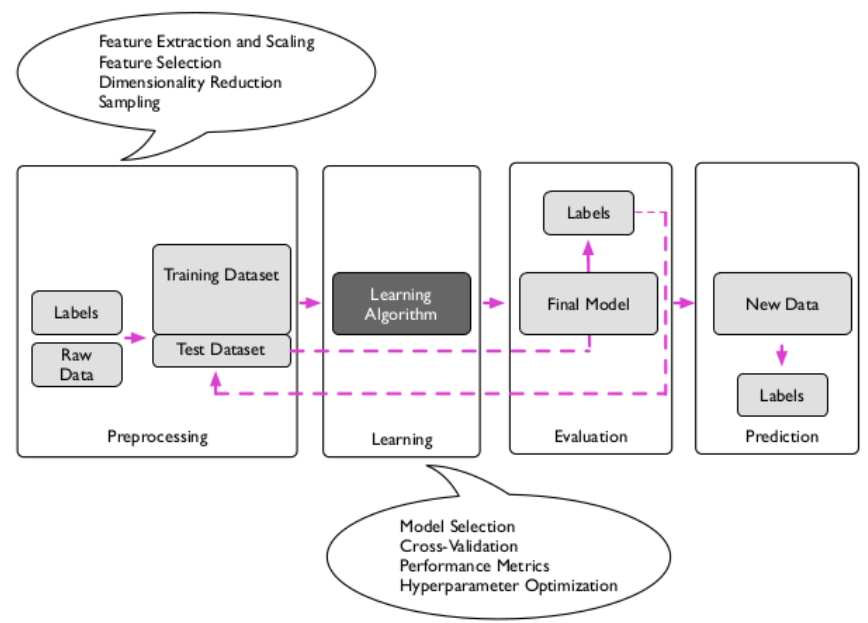
\includegraphics[width=0.75\textwidth]{../figures/overview_supervised_learning_process.png}
		\caption{Roadmap for building ML systems. Source: \citep[p. 11]{raschka2019PythonMachineLearning}.}
	\end{figure}
\end{frame}

\begin{frame}[fragile]{References}
	\begin{itemize}
		\small
		\setlength{\itemsep}{0.15cm}
		\item \citet{Bishop2016} --- Pattern Recognition and Machine Learning (PRML)
		\item \citet{james2023IntroductionStatisticalLearning} --- Introduction to Statistical Learning (ISL)
		\item \citet{hastieElementsStatisticalLearning2009} --- Elements of Statistical Learning (ESL)
		%\item \citet{mullainathan2017MachineLearningApplied} --- Machine Learning: An Applied Econometric Approach
		\item \citet{raschka2019PythonMachineLearning} --- Python Machine Learning
		\item \citet{yu2024VeridicalDataScience} --- Veridical Data Science: The Practice of Responsible Data Analysis and Decision Making
		      % TODO: VERIFY - athey2019MachineLearningMethods may not be in library.bib
		\item Athey \& Wager (2019) --- Machine Learning Methods for Economists
		%\item Gretl User-Contributed Packages: \url{https://gretl.sourceforge.net/cgi-bin/gretldata.cgi?opt=SHOW_FUNCS}
		%\item Permutation Importance Package: \url{https://github.com/atecon/permutation_importance}
		%\item Gretl Manual: \url{https://gretl.sourceforge.net/}
	\end{itemize}
\end{frame}

% ==================== SECTION 1: MOTIVATION & CONTEXT ====================

\section{Introduction: What is Machine Learning?}

\begin{frame}
	\begin{center}
		\Large
		Motivation and Context\\
		\vspace{0.5cm}
		\normalsize
		Why Machine Learning for Economics?
	\end{center}
\end{frame}

\begin{frame}[fragile]{What is Machine Learning?}
	\begin{block}{Definition}
		Machine learning refers to a set of computational methods that \textbf{learn from data} without being explicitly programmed. The system improves its performance on a given task through experience.
	\end{block}

	\vspace{0.3cm}

	\textbf{Three Learning Paradigms:}
	\begin{enumerate}
		\setlength{\itemsep}{0.2cm}
		\item \textbf{Supervised Learning}: Learn from labeled data with known output signals (labels)
		      \begin{itemize}
			      \small
			      \item Regression (continuous output), Classification (discrete output)
		      \end{itemize}
		\item \textbf{Unsupervised Learning}: Find patterns in unlabeled data
		      \begin{itemize}
			      \small
			      \item Clustering, Dimensionality reduction
		      \end{itemize}
		\item \textbf{Reinforcement Learning}: Learn through interaction and rewards
		      \begin{itemize}
			      \small
			      \item Not covered in this seminar
		      \end{itemize}
	\end{enumerate}
\end{frame}

\begin{frame}[fragile]{ML vs. Statistics vs. Econometrics}
	\begin{table}
		\small
		\setlength{\tabcolsep}{4pt}
		\renewcommand{\arraystretch}{1.15}
		\begin{tabular}{|p{0.20\textwidth}|p{0.23\textwidth}|p{0.23\textwidth}|p{0.23\textwidth}|}
			\hline
			\textbf{Dimension} & \textbf{Statistics}   & \textbf{ML}      & \textbf{Econometrics}    \\
			\hline
			Primary Goal       & Inference             & Prediction       & Causal Inference         \\
			\hline
			Focus              & Population parameters & Generalization   & Structural relationships \\
			\hline
			Uncertainty        & $p$-values, CI        & Validation error & Significance tests       \\
			\hline
			Assumptions        & Rigid                 & Flexible         & Economic theory          \\
			\hline
			Interpretability   & Essential             & Optional         & Critical                 \\
			\hline
			Data Dimension     & Low-medium            & High             & Low-medium               \\
			\hline
		\end{tabular}
	\end{table}

	\vspace{0.3cm}
	\textbf{Key insight:} \textit{Good prediction requires controlling overfitting and model complexity, not just fitting the observed data well.}
\end{frame}

\begin{frame}[fragile]{Why ML for Economics?}
	\begin{itemize}
		\setlength{\itemsep}{0.3cm}
		\item \textbf{High-dimensional problems}: Modern datasets have many features
		      \begin{itemize}
			      \small
			      \item Example: Predicting firm defaults with hundreds of financial indicators
		      \end{itemize}
		\item \textbf{Nonlinear relationships}: Economic phenomena often lack linearity
		      \begin{itemize}
			      \small
			      \item Example: Household consumption behavior with interaction effects
		      \end{itemize}
		\item \textbf{Model selection}: Regularization helps choose among competing specifications
		      \begin{itemize}
			      \small
			      \item Replaces ad-hoc variable selection with automatic methods
		      \end{itemize}
		\item \textbf{Prediction accuracy}: Sometimes prediction matters more than understanding
		      \begin{itemize}
			      \small
			      \item Example: Forecasting macroeconomic variables for policy decisions
		      \end{itemize}
		\item \textbf{Causal ML}: Combines econometric theory with ML flexibility
		      \begin{itemize}
			      \small
			      \item Example: Heterogeneous treatment effects, policy evaluation
		      \end{itemize}
	\end{itemize}
\end{frame}


% \begin{frame}{Gretl for Machine Learning}
% 	\textbf{Strengths:}
% 	\begin{itemize}
% 		\setlength{\itemsep}{0.15cm}
% 		\item \textbf{Econometric focus}: Tailored for economic data and methods
% 		\item \textbf{Built-in methods}: Lack of ML approaches (mainly statistical and econometric methods) but growing
% 		\item \textbf{User packages}: Random Forest, KNN, KMeans, Ridge \& Lasso, SVM, etc.
% 		\item \textbf{Both for education and research}: Versatile tool for teaching and ``serious'' empirical analysis
% 		\item \textbf{Integration with R/Python/Julia}: Can call external scripts for advanced ML methods
% 		\item \textbf{Script-based}: Reproducibility and automation
% 		\item \textbf{Educational}: Clean interface, reproducible scripts
% 		\item \textbf{Open-source}: Transparent, modifiable code
% 	\end{itemize}

% 	\vspace{0.3cm}

% 	\textbf{Limitations:}
% 	\begin{itemize}
% 		\setlength{\itemsep}{0.15cm}
% 		\item \textbf{Less comprehensive} than scikit-learn (Python)
% 		\item \textbf{No deep learning} support natively
% 		\item \textbf{Smaller community} than mainstream ML frameworks
% 	\end{itemize}
% \end{frame}



% ==================== SECTION 2: SUPERVISED LEARNING - FOUNDATIONS ====================

\section{Supervised Learning: Foundations}

\begin{frame}
	\begin{center}
		\Large
		Supervised Learning\\
		\vspace{0.5cm}
		\normalsize
		Core Concepts and Methods
	\end{center}
\end{frame}

\begin{frame}[fragile]{Regression vs. Classification}
	\textbf{Supervised Learning Problem:}
	\[
		y = f(\mathbf{X}) + \varepsilon
	\]
	where $\mathbf{X} = (X_1, \ldots, X_p)$ are features/predictors and $y$ is the target/response.

	\vspace{0.3cm}

	\begin{columns}
		\column{0.5\textwidth}
		\textbf{Regression}
		\begin{itemize}
			\setlength{\itemsep}{0.15cm}
			\item $y \in \mathbb{R}$ (continuous)
			\item Goal: Predict a real number
			\item Example: House prices, GDP growth
			\item Error: MSE, MAE, RMSE
		\end{itemize}

		\column{0.5\textwidth}
		\textbf{Classification}
		\begin{itemize}
			\setlength{\itemsep}{0.15cm}
			\item $y \in \{0, 1, \ldots, K-1\}$ (discrete)
			\item Goal: Predict a category
			\item Example: Default/no default, recession/no recession
			\item Error: Misclassification rate, AUC
		\end{itemize}
	\end{columns}
\end{frame}

\begin{frame}[fragile]{Training, Validation, and Test Data}
	\textbf{Standard procedure to estimate generalization error:}

	\vspace{0.3cm}

	\begin{enumerate}
		\setlength{\itemsep}{0.25cm}
		\item \textbf{Training Set} ($\sim 70\%$ of data)
		      \begin{itemize}
			      \small
			      \item Fit all candidate models here
			      \item Choose model complexity (e.g., $\lambda$) via validation error
		      \end{itemize}
		\item \textbf{Validation Set} ($\sim 15\%$ of data)
		      \begin{itemize}
			      \small
			      \item Tune hyperparameters (e.g., regularization parameter)
			      \item Select among candidate models
		      \end{itemize}
		\item \textbf{Test Set} ($\sim 15\%$ of data)
		      \begin{itemize}
			      \small
			      \item \textbf{Never touch during training}
			      \item Report final performance here
			      \item Represents future unseen data
		      \end{itemize}
	\end{enumerate}

	\vspace{0.3cm}

	\textbf{Why?} Training error is overly optimistic due to overfitting. Test error is the real performance metric.
\end{frame}


\begin{frame}[fragile]{Bias-Variance Tradeoff: Visual Example}

	\textbf{Variance}: Consistency of the model prediction for a data point if we would retrain the model multiple times on different subsets of the training data. $\Rightarrow$ Sensitivity to randomness in the data.
	\medskip

	\textbf{Bias}: Distance of the average prediction of the model from the true value we want to predict. $\Rightarrow$ Systematic error not due to randomness but due to model assumptions.

	\begin{figure}
		\centering
		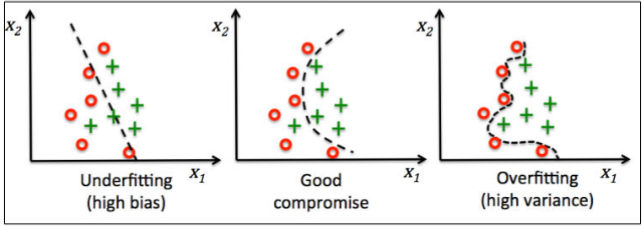
\includegraphics[width=0.8\textwidth]{../figures/raschka2019_classification_underfitting_overfitting.png}
		\caption{Example of underfitting (high bias), good fit (balanced), and overfitting (high variance). Source: \citep[p. 66]{raschka2019PythonMachineLearning}.}
	\end{figure}
\end{frame}


\begin{frame}[fragile]{Bias-Variance Tradeoff}
	\textbf{Test error (expected loss) decomposition:} \citep[pp. 148]{Bishop2016}
	\[
		\text{Test Error} = \underbrace{\text{Bias}^2}_{\text{underfitting}} + \underbrace{\text{Variance}}_{\text{overfitting}} + \underbrace{\text{Irreducible Error}}_{\text{noise}}
	\]

	\vspace{0.3cm}

	\begin{itemize}
		\setlength{\itemsep}{0.2cm}
		\item \textbf{High Bias}: Model too simple, cannot capture true relationship
		      \begin{itemize}
			      \small
			      \item Linear regression on nonlinear data
		      \end{itemize}
		\item \textbf{High Variance}: Model too flexible, fits noise in training data
		      \begin{itemize}
			      \small
			      \item Very deep decision tree overfitting training data
		      \end{itemize}
		\item \textbf{Objective}: Minimize expected loss
		\item \textbf{Problem}: Tradeoff between bias and variance --- reducing one often increases the other
		\item \textbf{Goal}: Balance --- find ``sweet spot'' complexity
	\end{itemize}
\end{frame}

\section{OLS, Ridge and Lasso}


\begin{frame}
	\begin{center}
		\Large
		OLS, Ridge, and Lasso Regression\\
	\end{center}
\end{frame}


\begin{frame}{OLS}
	\begin{equation}
		\min_{\boldsymbol{\beta}} \frac{1}{n} \sum_{i=1}^n (y_i - \mathbf{x}_i^\top \boldsymbol{\beta})^2
	\end{equation}

	\begin{itemize}
		\setlength{\itemsep}{0.2cm}
		\item Baseline linear model
		\item No regularization --- fits training data as closely as possible
		\item High bias if omitted variables are important; high variance with many features
		\item Solution: $\hat{\boldsymbol{\beta}} = (\mathbf{X}^\top \mathbf{X})^{-1} \mathbf{X}^\top \mathbf{y}$
	\end{itemize}

	\vspace{0.2cm}

	\textbf{When does OLS fail?}
	\begin{itemize}
		\small
		\item Many features ($p > n$): $\mathbf{X}^\top \mathbf{X}$ becomes singular
		\item Multicollinearity: Coefficients become large and unstable
	\end{itemize}
\end{frame}


\begin{frame}{Regularization: Ridge Regression (L2 Penalty)}
	\begin{equation}
		\min_{\boldsymbol{\beta}} \frac{1}{n} \sum_{i=1}^n (y_i - \mathbf{x}_i^\top \boldsymbol{\beta})^2
		+ \underbrace{\lambda \sum_{j=1}^p \beta_j^2}_{\text{L2 penalty}}
	\end{equation}
	%\vspace{0.2cm}

	\begin{columns}[T,onlytextwidth]
		\column{0.5\textwidth}
		\begin{itemize}
			\item \textbf{Penalty term}: shrinks coefficients in contrast to discrete variable selection
			\item \textbf{Tuning parameter} $\lambda \geq 0$ controls shrinkage strength
			\item $\lambda = 0 \Rightarrow$ OLS; $\lambda \to \infty \Rightarrow \beta_j \to 0$
			\item Reduces variance at the cost of small bias
			\item \textbf{No feature selection}: coefficients are typically not set to zero
		\end{itemize}

		\column{0.5\textwidth}
		\begin{figure}
			\centering
			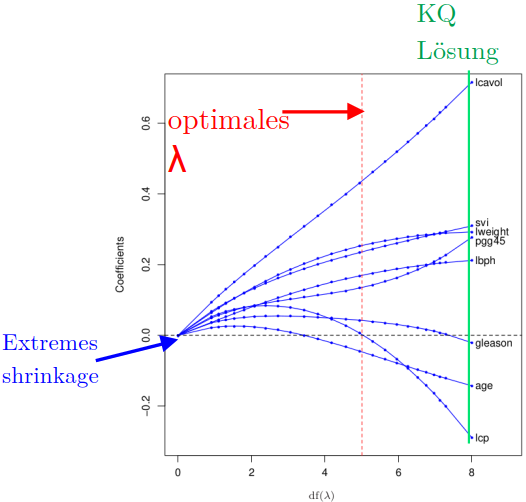
\includegraphics[width=0.95\textwidth]{../figures/ridge_path_coefficient.png}
		\end{figure}
	\end{columns}
\end{frame}

\begin{frame}{Regularization: Lasso Regression (L1 Penalty)}
	\begin{equation}
		\min_{\boldsymbol{\beta}} \frac{1}{n} \sum_{i=1}^n (y_i - \mathbf{x}_i^\top \boldsymbol{\beta})^2
		+ \underbrace{\lambda \sum_{j=1}^p |\beta_j|}_{\text{L1 penalty}}
	\end{equation}

	\begin{columns}[T,onlytextwidth]
		\column{0.55\textwidth}
		\begin{itemize}
			\item \textbf{Penalty term}: L1 norm, not squared
			\item \textbf{Key difference from Ridge}: Induces \textbf{sparsity}
			\item Some coefficients shrunk \textbf{exactly to zero} --- automatic feature selection
			\item Lasso can be inconsistent in feature selection \citep{zou2006AdaptiveLassoIts} -- adaptive lasso can fix this
			\item Useful for high-dimensional problems ($p \gg n$)
		\end{itemize}

		\column{0.45\textwidth}
		\begin{figure}
			\centering
			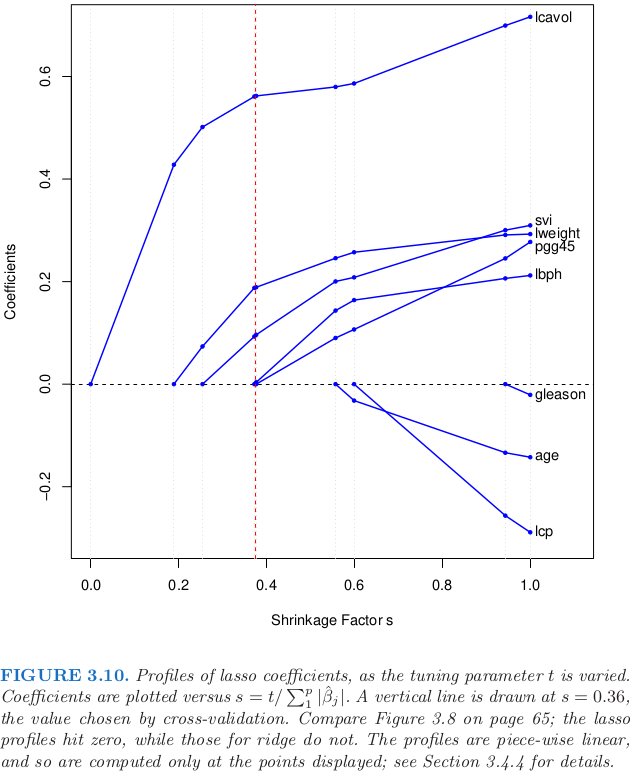
\includegraphics[width=0.88\textwidth]{../figures/james_etal_lasso_coefficient_path.png}
		\end{figure}
	\end{columns}
\end{frame}

\begin{frame}[fragile]{Gretl Packages for Regularized Regression}
	\textbf{Gretl packages}
	\begin{itemize}
		\setlength{\itemsep}{0.18cm}
		\item \texttt{regls}: Add-on for Ridge and Lasso regression (Allin Cottrell).\\
			  Doc: \url{https://sourceforge.net/projects/gretl/files/addons/doc/regls.pdf}
		\item \texttt{graphlasso}: Graphical Lasso (Sven Schreiber).\\
			  Doc: \url{https://gretl.sourceforge.net/current_fnfiles/graphlasso.gfn}
		\item \texttt{adalasso}: Adaptive Lasso (Sven Schreiber).\\
			  Doc: \url{https://gretl.sourceforge.net/current_fnfiles/adalasso.gfn}
		\item \texttt{fsboost}: Forward-stagewise boosted regression estimates (Artur Tarassow).\\
			  Doc: \url{https://gretl.sourceforge.net/current_fnfiles/unzipped/fsboost.pdf}
	\end{itemize}
\end{frame}

% \begin{frame}{OLS vs. Ridge vs. Lasso: Comparison}
% 	\begin{table}
% 		\tiny
% 		\begin{tabular}{|l|c|c|c|}
% 			\hline
% 			\textbf{Aspect}   & \textbf{OLS}          & \textbf{Ridge}           & \textbf{Lasso}                \\
% 			\hline
% 			Penalty           & None                  & $\lambda \beta_j^2$      & $\lambda |\beta_j|$           \\
% 			\hline
% 			Feature Selection & No                    & No                       & Yes (sparse)                  \\
% 			\hline
% 			Bias              & None                  & Small positive           & Small positive                \\
% 			\hline
% 			Variance          & High (many features)  & Lower                    & Lower                         \\
% 			\hline
% 			When to use       & Few features, low $p$ & Many correlated features & Many features, want selection \\
% 			\hline
% 			Interpretability  & High                  & High                     & High (fewer features)         \\
% 			\hline
% 		\end{tabular}
% 	\end{table}

% 	\vspace{0.2cm}
% 	\textbf{Elastic Net:} Combines Ridge and Lasso penalties: $\lambda_1 \sum |\beta_j| + \lambda_2 \sum \beta_j^2$
% \end{frame}




\begin{frame}{Code Example 1: OLS, Ridge, and Lasso in Gretl}
	See code examples:
	\vspace{0.25cm}

	\begin{itemize}
		\setlength{\itemsep}{0.15cm}
		\item \texttt{ridge\_lasso\_coefficient\_path.inp}: Coefficient paths for Ridge and Lasso using the \texttt{regls} package
		\item \texttt{crossval\_ridge\_lasso.inp}: Cross-validation to select $\lambda$ for Ridge and Lasso
	\end{itemize}
\end{frame}


\section{K-Nearest Neighbors}

\begin{frame}
	\begin{center}
		\Large
		K-Nearest Neighbors (KNN)
	\end{center}
\end{frame}

\begin{frame}{K-Nearest Neighbors (KNN): Lazy Learning}
    \begin{itemize}
        \item Popular non-parametric approach in machine learning.
        \item \textit{Lazy learner}: it does not learn an explicit function but memorizes the training dataset (\textit{instance-based learner}).
        \item Basic idea: similar data points (features) should have similar outcomes (target values).
        \item Identifies the $K$ points in the training data that are closest to a new point $x_q$ (query).
        \item \textbf{Advantage} of the memory-based approach: the model immediately adapts to new data as soon as it becomes available.
        \item \textbf{Disadvantage}: Computational complexity increases linearly with $n^{train}$.
    \end{itemize}
\end{frame}

\begin{frame}{The Algorithm -- Illustrated for $K=1$ closest neighbor}
    %\small
    \begin{columns}
        \begin{column}{0.55\textwidth}
            Training dataset $\mathcal{D}$: $\{ \mathbf{x}_i, y_i \} \in \mathcal{D} \quad (|\mathcal{D}| = n)$\\
            New point:  $\{ \mathbf{x}_q, ??? \} \qquad $ (query point)\\
            Prediction: $f(\mathbf{x}_q)$
            \medskip

            \textbf{Algorithm}
            \small

            closest\_point $=$ none\\
            closest\_distance $ = \infty$

            \begin{enumerate}
                \item for $i=1,\ldots, n$
                      \begin{enumerate}\setcounter{enumii}{1}
                          \item current\_distance $= d(\mathbf{x}_i, \mathbf{x}_q)$
                          \item if current\_distance $<$ closest\_distance
                                \begin{enumerate}\setcounter{enumiii}{3}
                                    \item closest\_distance = current\_distance
                                    \item closest\_point = $\mathbf{x}_i$
                                \end{enumerate}
                      \end{enumerate}
                      \setcounter{enumi}{5}
                \item return $f(closest\_points)$ in the space $\mathcal{D}_k$.
            \end{enumerate}
        \end{column}
        \begin{column}{0.45\textwidth}  %%<--- here
            \begin{figure}
                \centering
                \subfigure{
                    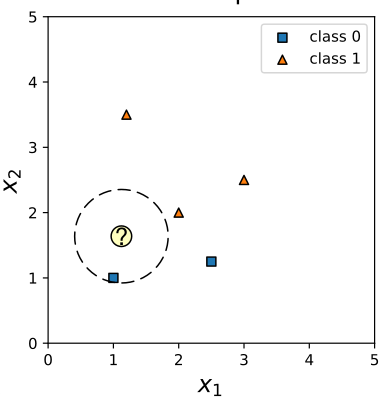
\includegraphics[width=.82\textwidth]{../figures/knn_1_circle.png}}
                \caption{\footnotesize Search for the nearest data point in the training dataset ($n=5$) which looks most "similar" using some distance function $d()$.}
                %\label{fig:kmeans_steps}
            \end{figure}
        \end{column}
    \end{columns}
\end{frame}


\begin{frame}{Prediction for query point $\mathbf{x}_q$}
	\begin{itemize}
		\setlength{\itemsep}{0.2cm}
		\item For a new observation $\mathbf{x}_0$, find the $k$ closest observations in training data
		      \begin{itemize}
			      \small
			      \item Distance metric: Usually Euclidean: $d(\mathbf{x}_q, \mathbf{x}_i) = \sqrt{\sum_j (x_{qj } - x_{ij})^2}$
		      \end{itemize}
		\item \textbf{For classification}: Majority vote among $k$ neighbors
		      \begin{itemize}
			      \small
			      \item $\hat{y}_0 = \text{mode}(y_1, \ldots, y_k)$
		      \end{itemize}
		\item \textbf{For regression}: Average the $k$ neighbors
		      \begin{itemize}
			      \small
			      \item $\hat{y}_0 = \frac{1}{k} \sum_{i=1}^k y_i$
		      \end{itemize}
	\end{itemize}

	\vspace{0.2cm}

	\textbf{Hyperparameter:} $k$ (number of neighbors)
	\begin{itemize}
		\small
		\item Small $k$ (e.g., 1): Flexible, high variance, overfitting risk
		\item Large $k$ (e.g., $n$): Inflexible, high bias, underfitting risk
		\item Typically selected via cross-validation
	\end{itemize}
\end{frame}

\begin{frame}[fragile]{KNN: Advantages and Disadvantages}
	\textbf{Advantages:}
	\begin{itemize}
		\setlength{\itemsep}{0.15cm}
		\item Simple and intuitive
		\item No assumptions about data distribution
		\item Works for both regression and classification
		\item Captures local patterns well
	\end{itemize}

	\vspace{0.2cm}

	\textbf{Disadvantages:}
	\begin{itemize}
		\setlength{\itemsep}{0.15cm}
		\item \textbf{Curse of dimensionality}: Distance becomes less meaningful with many features
		\item Computational cost: Must compute distance to all training points for each prediction
		\item Sensitive to feature scaling --- requires standardization
		\item Poor interpretability --- why did we classify this way?
	\end{itemize}
\end{frame}

\begin{frame}{Class separability \& Hyperparameter Tuning Using CV}
	\small
	\begin{figure}
		\centering
		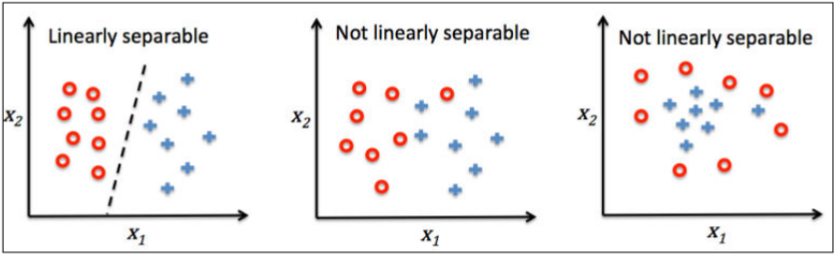
\includegraphics[width=0.5\textwidth]{../figures/raschka2019_classification_linear_nonlinear_separability.png}
		\caption{Linear vs. non-linear separability. Source: \citep[p. 23]{raschka2019PythonMachineLearning}.}
	\end{figure}
	\vspace{-0.7cm}
	%\begin{figure}
	%	\centering
	%	\includegraphics[width=0.425\textwidth]{../figures/knn_decision_boundaries.png}
	%	\caption{KNN decision boundary example. Source: \citep[p. 54]{raschka2019PythonMachineLearning}.}
	%\end{figure}

	\begin{figure}
        \centering
        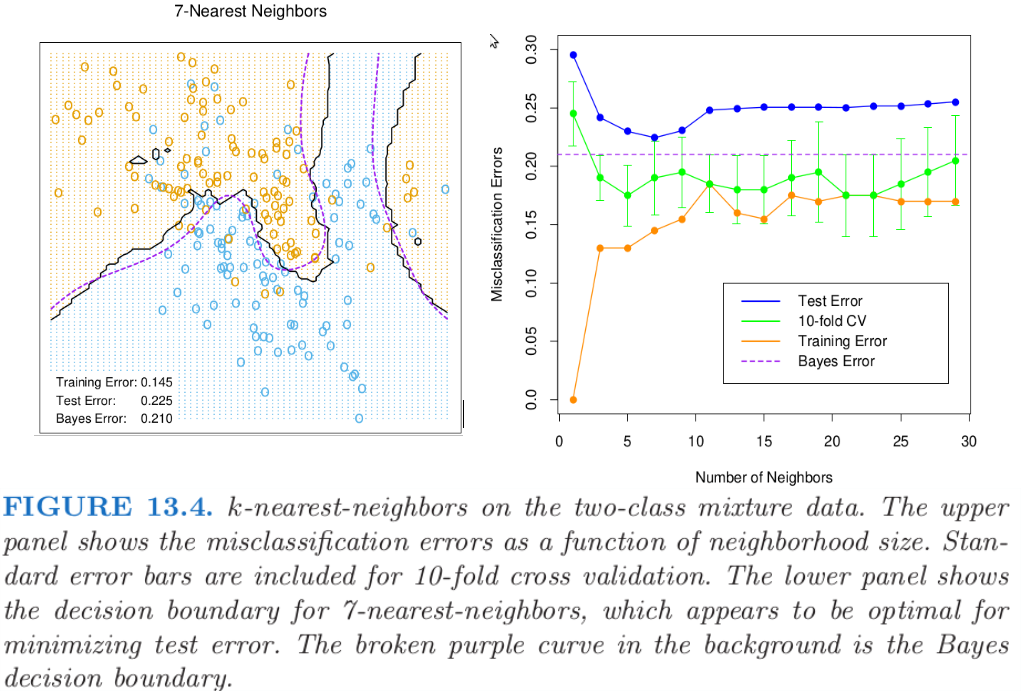
\includegraphics[width=.66\textwidth]{../figures/knn_example_James_etal2017.png}
        \caption{\footnotesize{Source: \citet[p. 467]{james2023IntroductionStatisticalLearning}}}
        %\label{fig:kmeans_mrw}
    \end{figure}
\end{frame}


\begin{frame}{KNN Using Time-Series Data}
    \begin{figure}
        \centering
        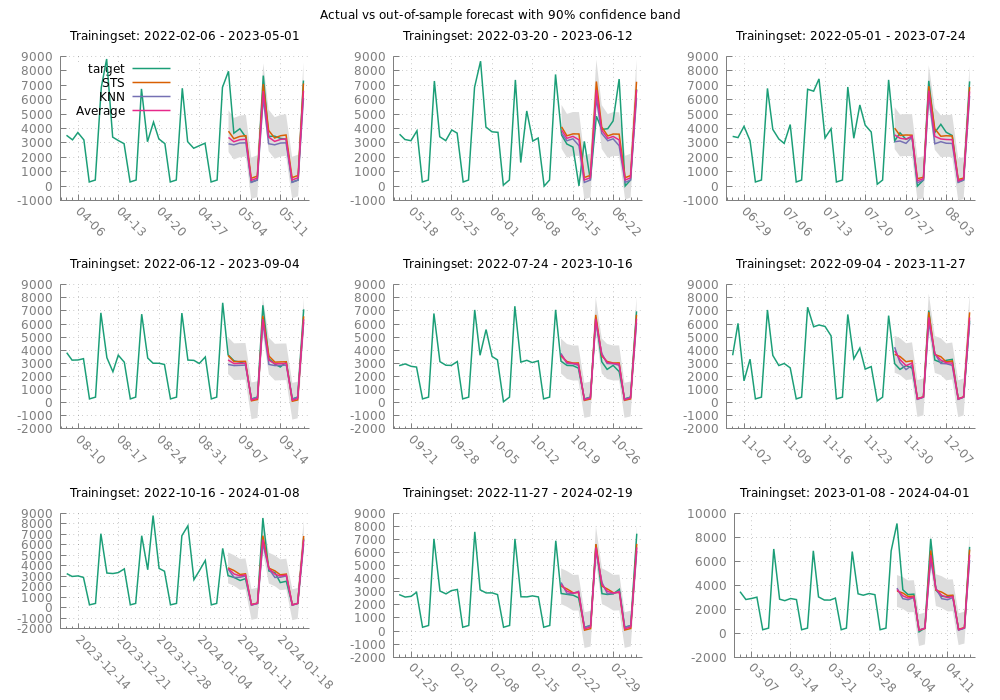
\includegraphics[width=0.7\textwidth]{../figures/forecasts_grid_unit=Kommi Kontaktlinse_window=450.png}
        \caption{\footnotesize \textit{Out-of-sample} ($h=14$ days) time-series forecasting using KNN, in comparison to a structural time-series model. Daily data with day features (e.g., day of week, holidays).}
    \end{figure}
\end{frame}


\begin{frame}{Gretl Package for KNN}
	\textbf{Package:} \texttt{knn.gfn} (Author: Artur Tarassow, v0.1, July 2024)

	\textbf{Main Features:}
	\begin{itemize}
		\setlength{\itemsep}{0.18cm}
		\item \textbf{Dual functionality:} Regression and binary/multi-class classification
		\item \textbf{Core functions:}
		      \begin{itemize}
			      \small
			      \item \texttt{knn\_fit()}: Fit KNN model to training data
			      \item \texttt{knn\_predict()}: Make predictions on test data
			      \item \texttt{knn\_scores()}: Calculate accuracy metrics
			      \item \texttt{knn\_summary()}: Print model summary
		      \end{itemize}
		\item \textbf{Distance metrics:} Various
		\item \textbf{Cross-validation:} K-fold, leave-one-out, recursive/rolling windows
	\end{itemize}
	\vspace{0.2cm}
	\textbf{Installation:} \texttt{pkg install knn}
\end{frame}


\begin{frame}{Code Example 2: KNN Classification in Gretl}
	See code examples:
	\vspace{0.25cm}

	\begin{itemize}
		\setlength{\itemsep}{0.15cm}
		\item \texttt{knn\_classification.inp}: KNN classification example using the \texttt{knn} package
	\end{itemize}
\end{frame}

% ==================== SECTION 3: TREE-BASED & KERNEL METHODS ====================

\section{Supervised Learning: Tree-Based and Kernel Methods}

\begin{frame}
	\begin{center}
		\Large
		Tree-Based Methods\\
		\vspace{0.5cm}
		\normalsize
		Decision Trees, Random Forests, and Beyond
	\end{center}
\end{frame}

\begin{frame}{Motivation}
	\begin{itemize}
		\item Tree-based methods as the \textit{workhorse} of supervised machine learning
		\item Used for both \textbf{regression} and \textbf{classification}
		\item Flexible non-parametric approach to data analysis and prediction
		\item Recursive division of the feature space into regions (\textit{stratification}/\textit{segmentation})
		\item Rule-based approach --- \textbf{rules are learned by the algorithm}, not hard-coded
		\item Each region assigned a single prediction value
		\item Interpretable: Can be visualized and explained
		\item Lacking prediction accuracy for a \textit{single} tree but forms the basis for powerful ensemble methods (Random Forests, Gradient Boosting)
	\end{itemize}
\end{frame}


\begin{frame}{Decision Tree}
	\begin{columns}
		\begin{column}{0.5\textwidth}
			\begin {itemize}
			\item The tree learns a sequence of (binary) questions based on features to identify the target variable classes
			\item Each question is represented by a node in the tree
			\item The leaves of the tree represent the classes
			\item Categorical variables and numerical variables can be used for splitting
			\end{itemize}
		\end{column}
		\begin{column}{0.5\textwidth}
			\begin{figure}
				\centering
				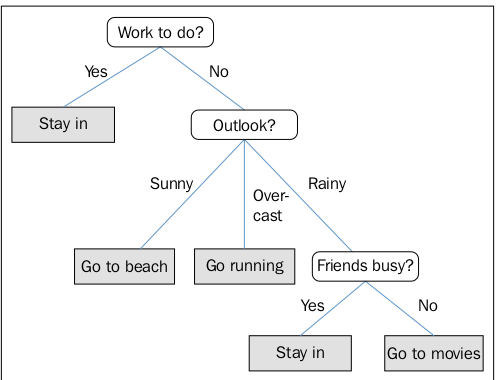
\includegraphics[width=.9\textwidth]{../figures/decision_tree_go_to_beach_from_raschka.png}
				\caption{\footnotesize Decision tree for day planning. Source: \citet{raschka2019PythonMachineLearning}}
			\end{figure}
		\end{column}
	\end{columns}
\end{frame}


\begin{frame}{Basic Concepts of Decision Trees}
	\begin{figure}
		\centering
		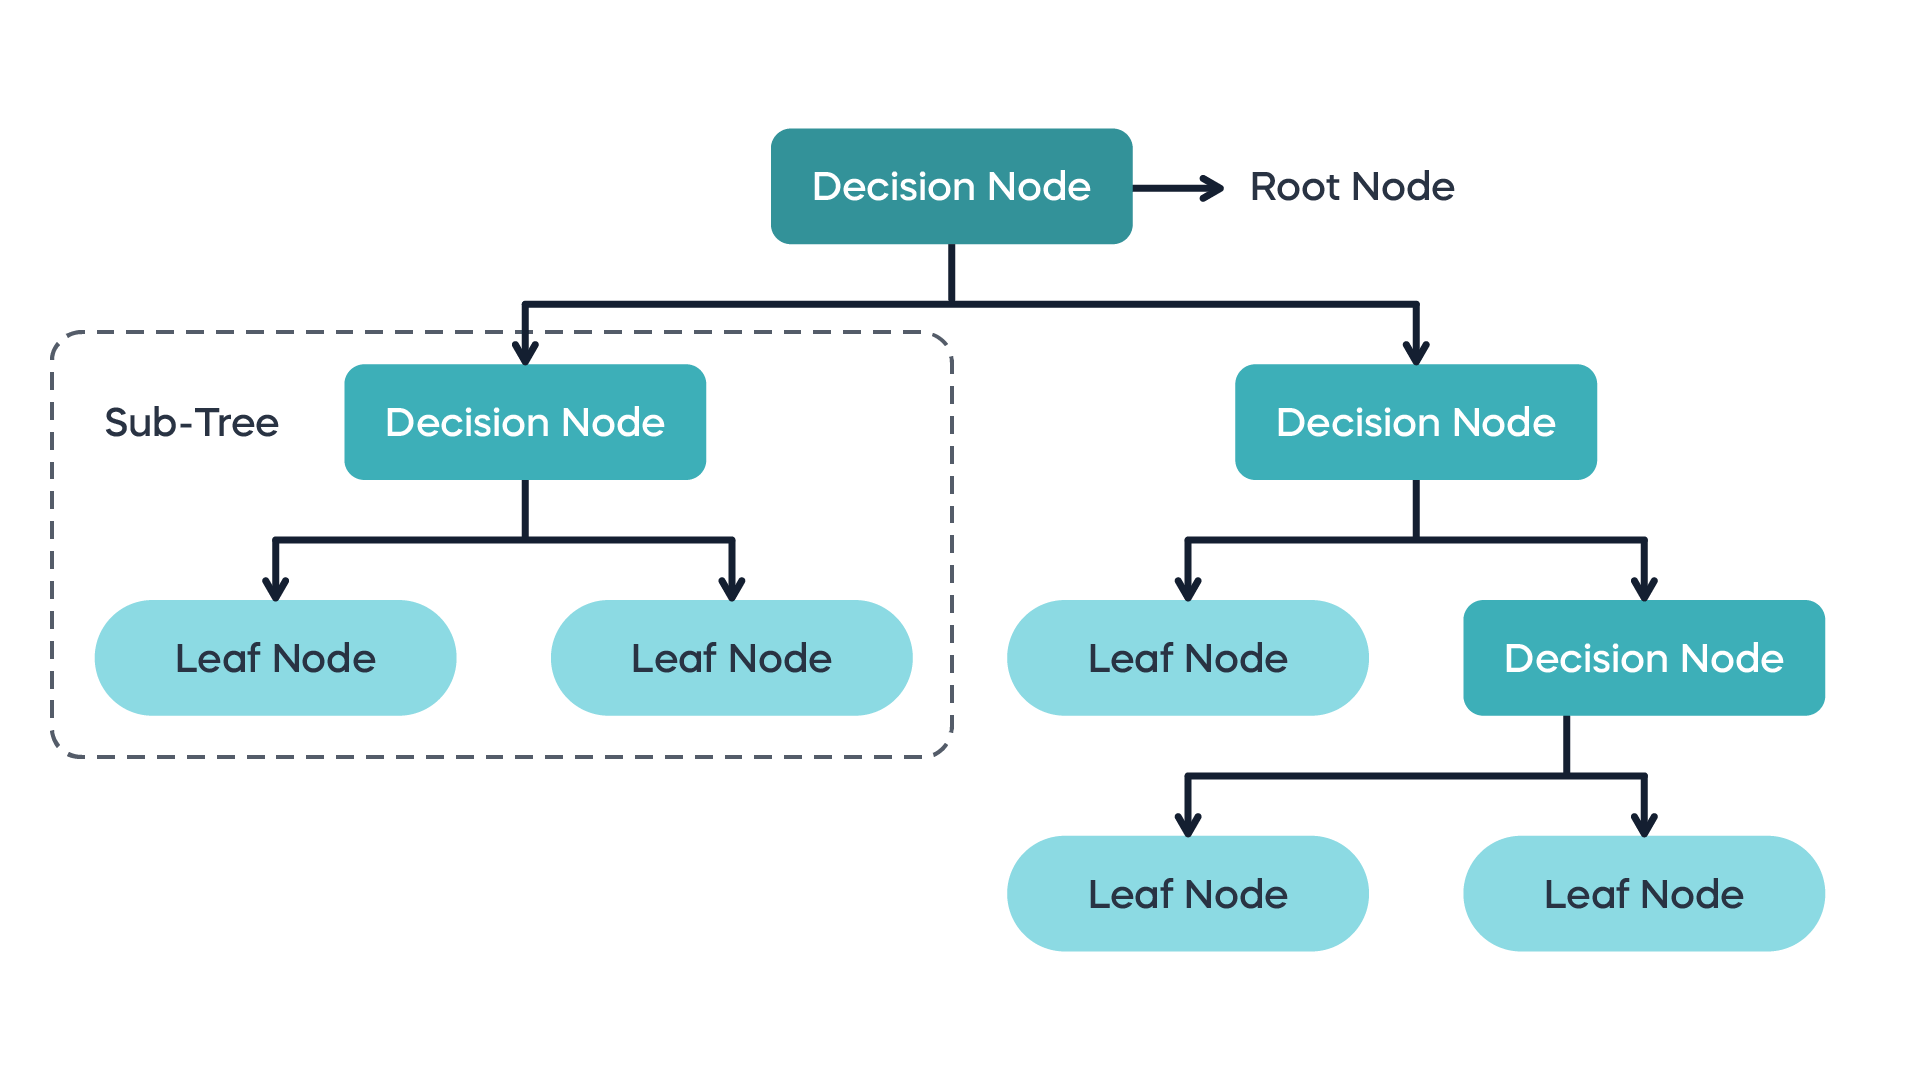
\includegraphics[width=.9\textwidth]{../figures/tree_basic_terminology.png}
		\caption{Connections between decision nodes are called \textbf{branches}.\newline \footnotesize Source: \url{https://365datascience.com/tutorials/machine-learning-tutorials/decision-trees/}}
	\end{figure}
\end{frame}


\begin{frame}{Example: Modeling Baseball Player Salaries \textbf{I}}
	\begin{columns}
		\begin{column}{0.5\textwidth}
			The CART algorithm is a popular method for building decision trees \citep{LeoBreiman.Stone1984}.
			\medskip

			\textbf{How it works:}
			\begin{enumerate}
				%\setlength{\itemsep}{0.15cm}
				\item Start with all data at root node
				\item Choose split on feature that best reduces impurity (Gini, entropy)
				\item Recursively split child nodes until stopping criterion
				\item Assign prediction based on majority (classification) or mean (regression)
			\end{enumerate}
		\end{column}

		\begin{column}{0.5\textwidth}
			\begin{figure}
				\centering
				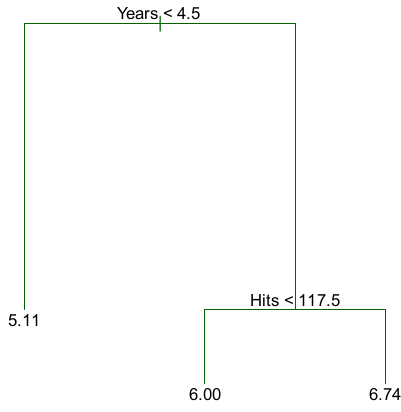
\includegraphics[width=.85\textwidth]{../figures/tree_basic_data=hitters.png}
				\caption{\footnotesize Binary tree with 2 internal nodes and 3 leaves. The value of each leaf corresponds to the average (logarithmic) salary of players in this partition.}
			\end{figure}
		\end{column}
	\end{columns}
\end{frame}

\begin{frame}{Example: Modeling Baseball Player Salaries \textbf{II}}
	\begin{columns}
		\begin{column}{0.5\textwidth}
			\begin{figure}
				\centering
				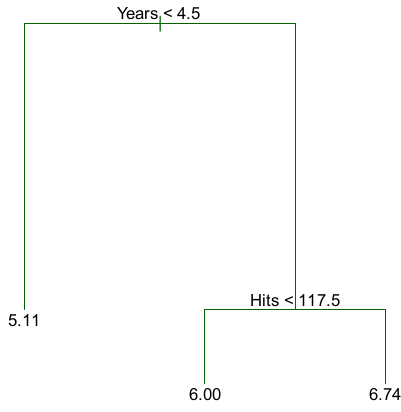
\includegraphics[width=.85\textwidth]{../figures/tree_basic_data=hitters.png}
				\caption{\footnotesize Players with less than 4.5 years of playing experience earn an average of $e^{5.11} = 165,000$ USD.}
				\label{fig:tree_hitters}
			\end{figure}
		\end{column}
		\begin{column}{0.5\textwidth}  %%<--- here
			\begin{figure}
				\centering
				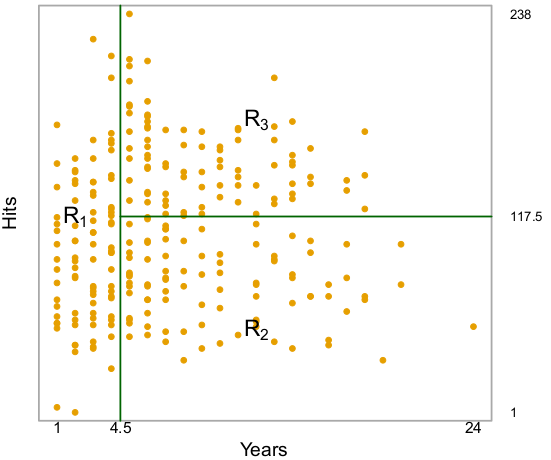
\includegraphics[width=.85\textwidth]{../figures/tree_basic_partiioned_space_data=hitters.png}
				\caption{\footnotesize The three regions of the input space defined by the tree in Fig. \ref{fig:tree_hitters}. This is the optimally \textit{pruned} tree with 3 terminal nodes.}
				\label{fig:tree_hitters_partitioned_space}
			\end{figure}
		\end{column}
	\end{columns}
\end{frame}


\begin{frame}[fragile]{Decision Trees: Splitting Criteria}
	\textbf{How to choose the best split?}\footnote{For details, see \citet{yu2024VeridicalDataScience}. URL: \url{https://vdsbook.com/12-rf}}

	\small

	\textbf{For Classification} --- minimize impurity:
	\begin{itemize}
		\setlength{\itemsep}{0.15cm}
		\item \textbf{Gini Impurity}: $G = 1 - \sum_{k=1}^K p_k^2$ (proportion of class $k$ in node)
		      \begin{itemize}
			      \small
			      \item Ranges 0 (pure, all one class) to $1 - 1/K$ (maximally mixed)
		      \end{itemize}
		\item \textbf{Entropy}: $H = -\sum_{k=1}^K p_k \log(p_k)$ (information theoretic)
		      \begin{itemize}
			      \small
			      \item Higher entropy = more uncertainty
		      \end{itemize}
	\end{itemize}

	\vspace{0.1cm}

	\textbf{For Regression} --- minimize within-node variance (look for similar $y$ values):
	\begin{itemize}
		\item For a split into left ($L$) and right ($R$) child nodes:
			  \[
				  \text{Var}_{\text{split}} = \frac{n_L}{n} \times \sigma_L^2 + \frac{n_R}{n} \times \sigma_R^2
			  \]
			  where $n_L$, $n_R$ are the number of observations in the left/right child nodes, $n = n_L + n_R$ is the parent node size, and $\sigma_L^2$, $\sigma_R^2$ are squared deviations from the mean in each child node, $\sigma^2 = \frac{1}{n} \sum_{i=1}^n (y_i - \bar{y})^2$.
	\end{itemize}
\end{frame}


\begin{frame}{Binary Classification Tree for a Purchase Decision}
	\begin{columns}
		\begin{column}{0.22\textwidth}
			\scriptsize
			A diagram depicting a decision tree for predicting purchase intent (a binary response). The tree has been trained on 30 training sessions, 8 of which ended with a purchase and are colored orange, and 22 of which did not and are colored blue.

			\href{https://vdsbook.com/12-rf\#fig-decision-tree-train-partition-example}{Source}
		\end{column}
		\begin{column}{0.78\textwidth}
			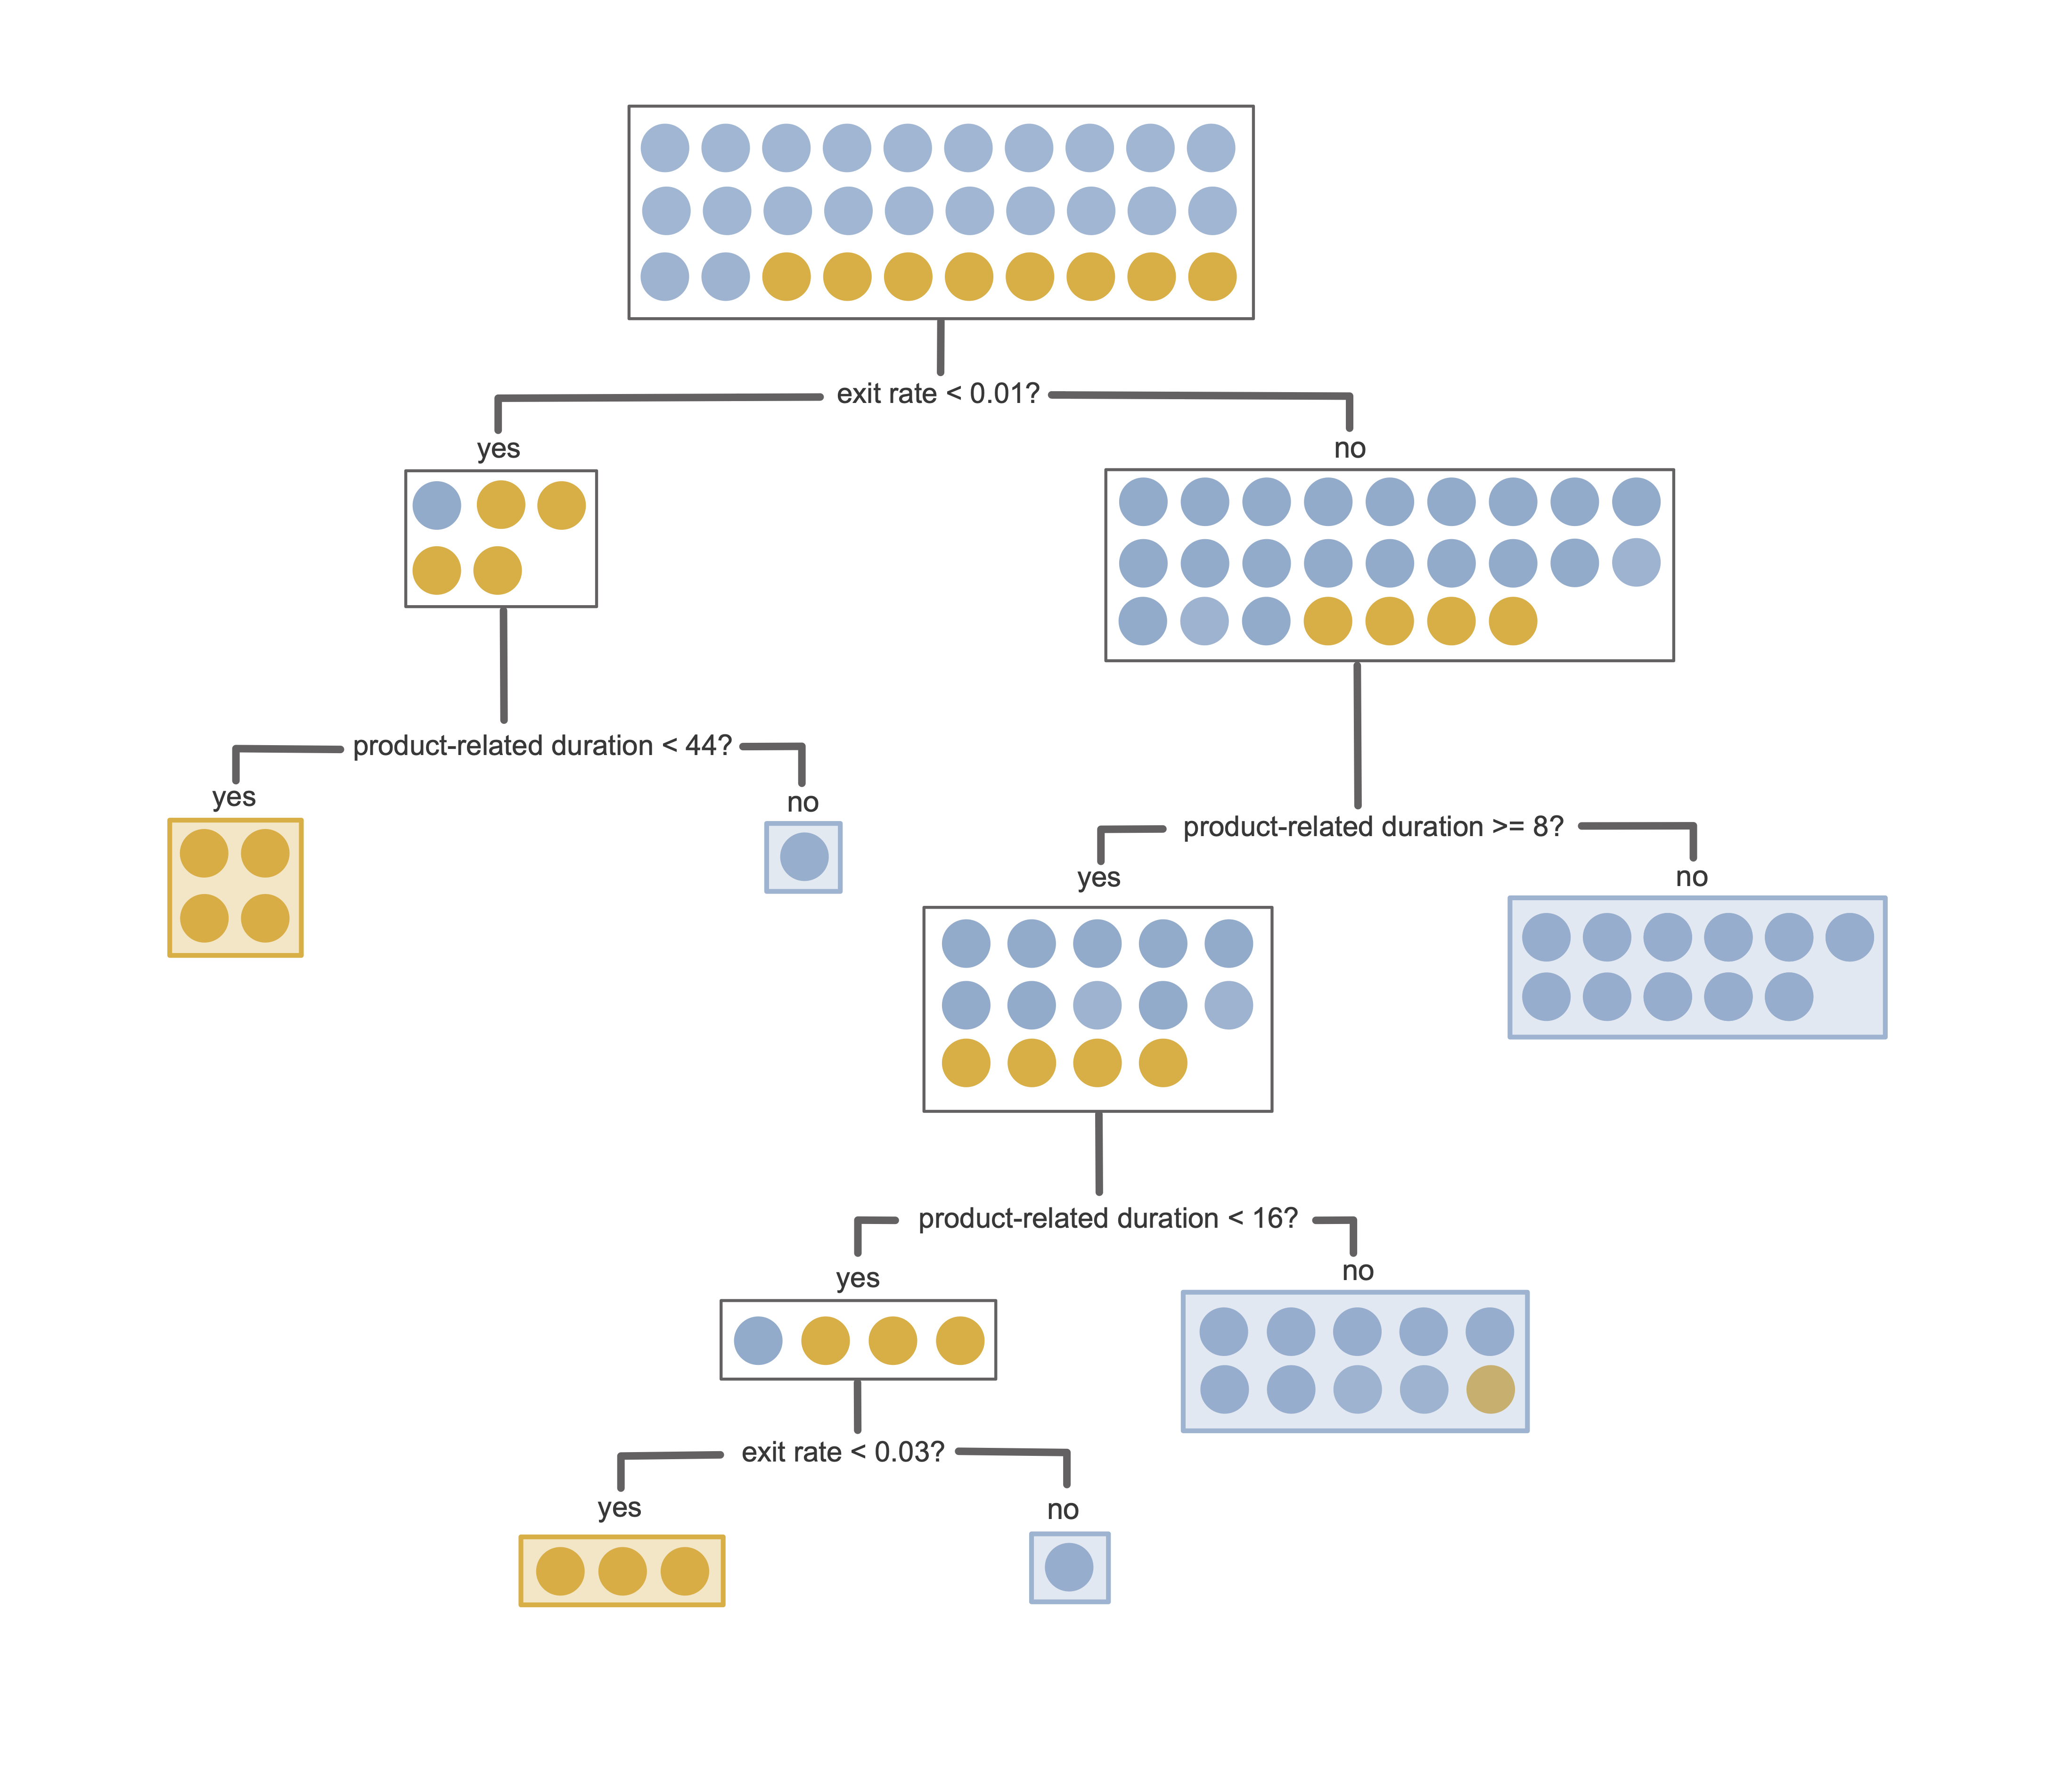
\includegraphics[width=\textwidth]{../figures/yu_barter_classification_tree.png}
		\end{column}
	\end{columns}
\end{frame}


\begin{frame}{Decision Trees: Overfitting and Pruning}
	\textbf{Problem:} Trees can grow very deep, fitting noise in training data
	\vspace{0.2cm}

	\begin{columns}
		\column{0.5\textwidth}
		\textbf{Unpruned Tree}
		\begin{itemize}
			\small
			\setlength{\itemsep}{0.15cm}
			\item Zero training error
			\item High test error (overfitting)
			\item Captures noise
		\end{itemize}

		\column{0.5\textwidth}
		\textbf{Pruned Tree}
		\begin{itemize}
			\small
			\setlength{\itemsep}{0.15cm}
			\item Small training error
			\item Lower test error (better generalization)
			\item Simpler, more interpretable
		\end{itemize}
	\end{columns}
	\vspace{0.5cm}

	\textbf{Key Hyperparameters (CART Algorithm):}
	\begin{table}
		\tiny
		\begin{tabular}{|l|c|c|c|}
			\hline
			\textbf{Hyperparameter} & \textbf{Description} & \textbf{R (rpart)} & \textbf{Python (sklearn)} \\
			\hline
			Maximum depth & Max number of sequential splits & \texttt{maxdepth} (default: 30) & \texttt{max\_depth} (no default) \\
			\hline
			Minimum node size & Min observations to split a node & \texttt{minsplit} (default: 20) & \texttt{min\_samples\_split} (default: 2) \\
			\hline
		\end{tabular}
	\end{table}
	%\vspace{0.1cm}
	%{\tiny \textbf{Note:} Tune via cross-validation; R defaults often work well in practice.}
\end{frame}

\begin{frame}{Comparison of Model Types}
	\begin{figure}
		\centering
		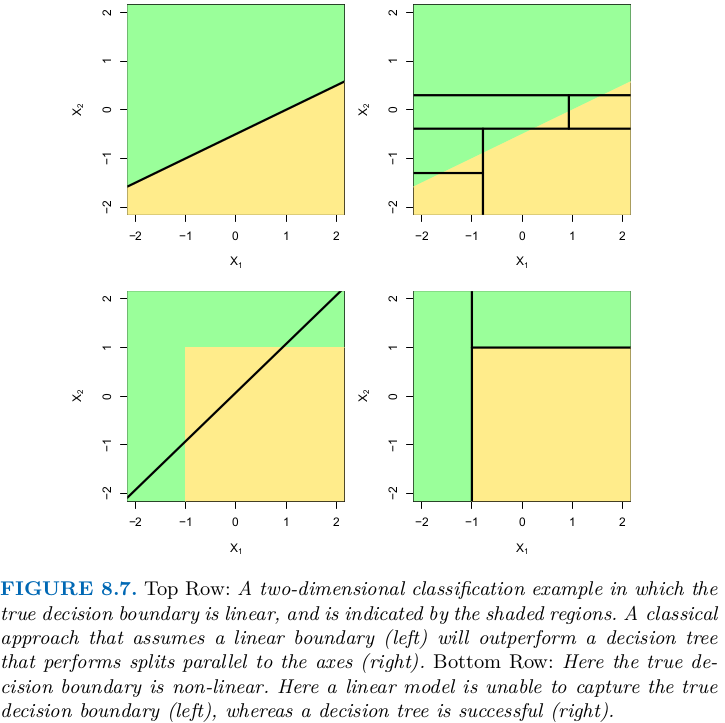
\includegraphics[width=.62\textwidth]{../figures/comparison_linearmodel_vs_treebased.png}
		%\caption{\texttt{Heart} dataset: Unpruned classification tree created through top-down recursive binary partitioning and \textit{greedy} splits.}
	\end{figure}
\end{frame}


\begin{frame}{Random Forests: Bootstrap Aggregation}
	\textbf{Problem} with single tree: High variance, overfitting
	\vspace{0.1cm}

	\textbf{Solution:} Grow many \textbf{decorrelated} trees and average (aggregate) their predictions \citep{breiman1996BaggingPredictors, breiman2001StatisticalModelingTwo}
	\vspace{0.2cm}

	\textbf{Algorithm:}
	\begin{enumerate}
		\setlength{\itemsep}{0.15cm}
		\item For $b = 1, \ldots, B$ (number of trees):
		      \begin{itemize}
			      \small
			      \item Draw bootstrap sample of size $n$ with replacement
			      \item Grow full tree on bootstrap sample (no pruning)
			      \item At each split, randomly select $m$ features from $p$ total
			            \begin{itemize}
				            \tiny
				            \item Typical: $m = \sqrt{p}$ for classification, $m = p/3$ for regression
			            \end{itemize}
		      \end{itemize}
		\item Average predictions across all $B$ trees:
			\vspace{0.1cm}

			\textbf{Classification (binary response):}
			\begin{itemize}
				\tiny
				\item \textit{Probability prediction}: Average of positive class probability predictions from individual trees
				\item \textit{Binary class prediction}: Majority vote of individual trees' binary predictions (or thresholded class probability)
			\end{itemize}
			\vspace{0.1cm}

			\item \textbf{Regression (continuous response)}: Mean prediction across all individual trees
	\end{enumerate}
\end{frame}


% New frame depicting RF example:
\begin{frame}{Random Forests: Illustration}
	\begin{figure}
		\centering
		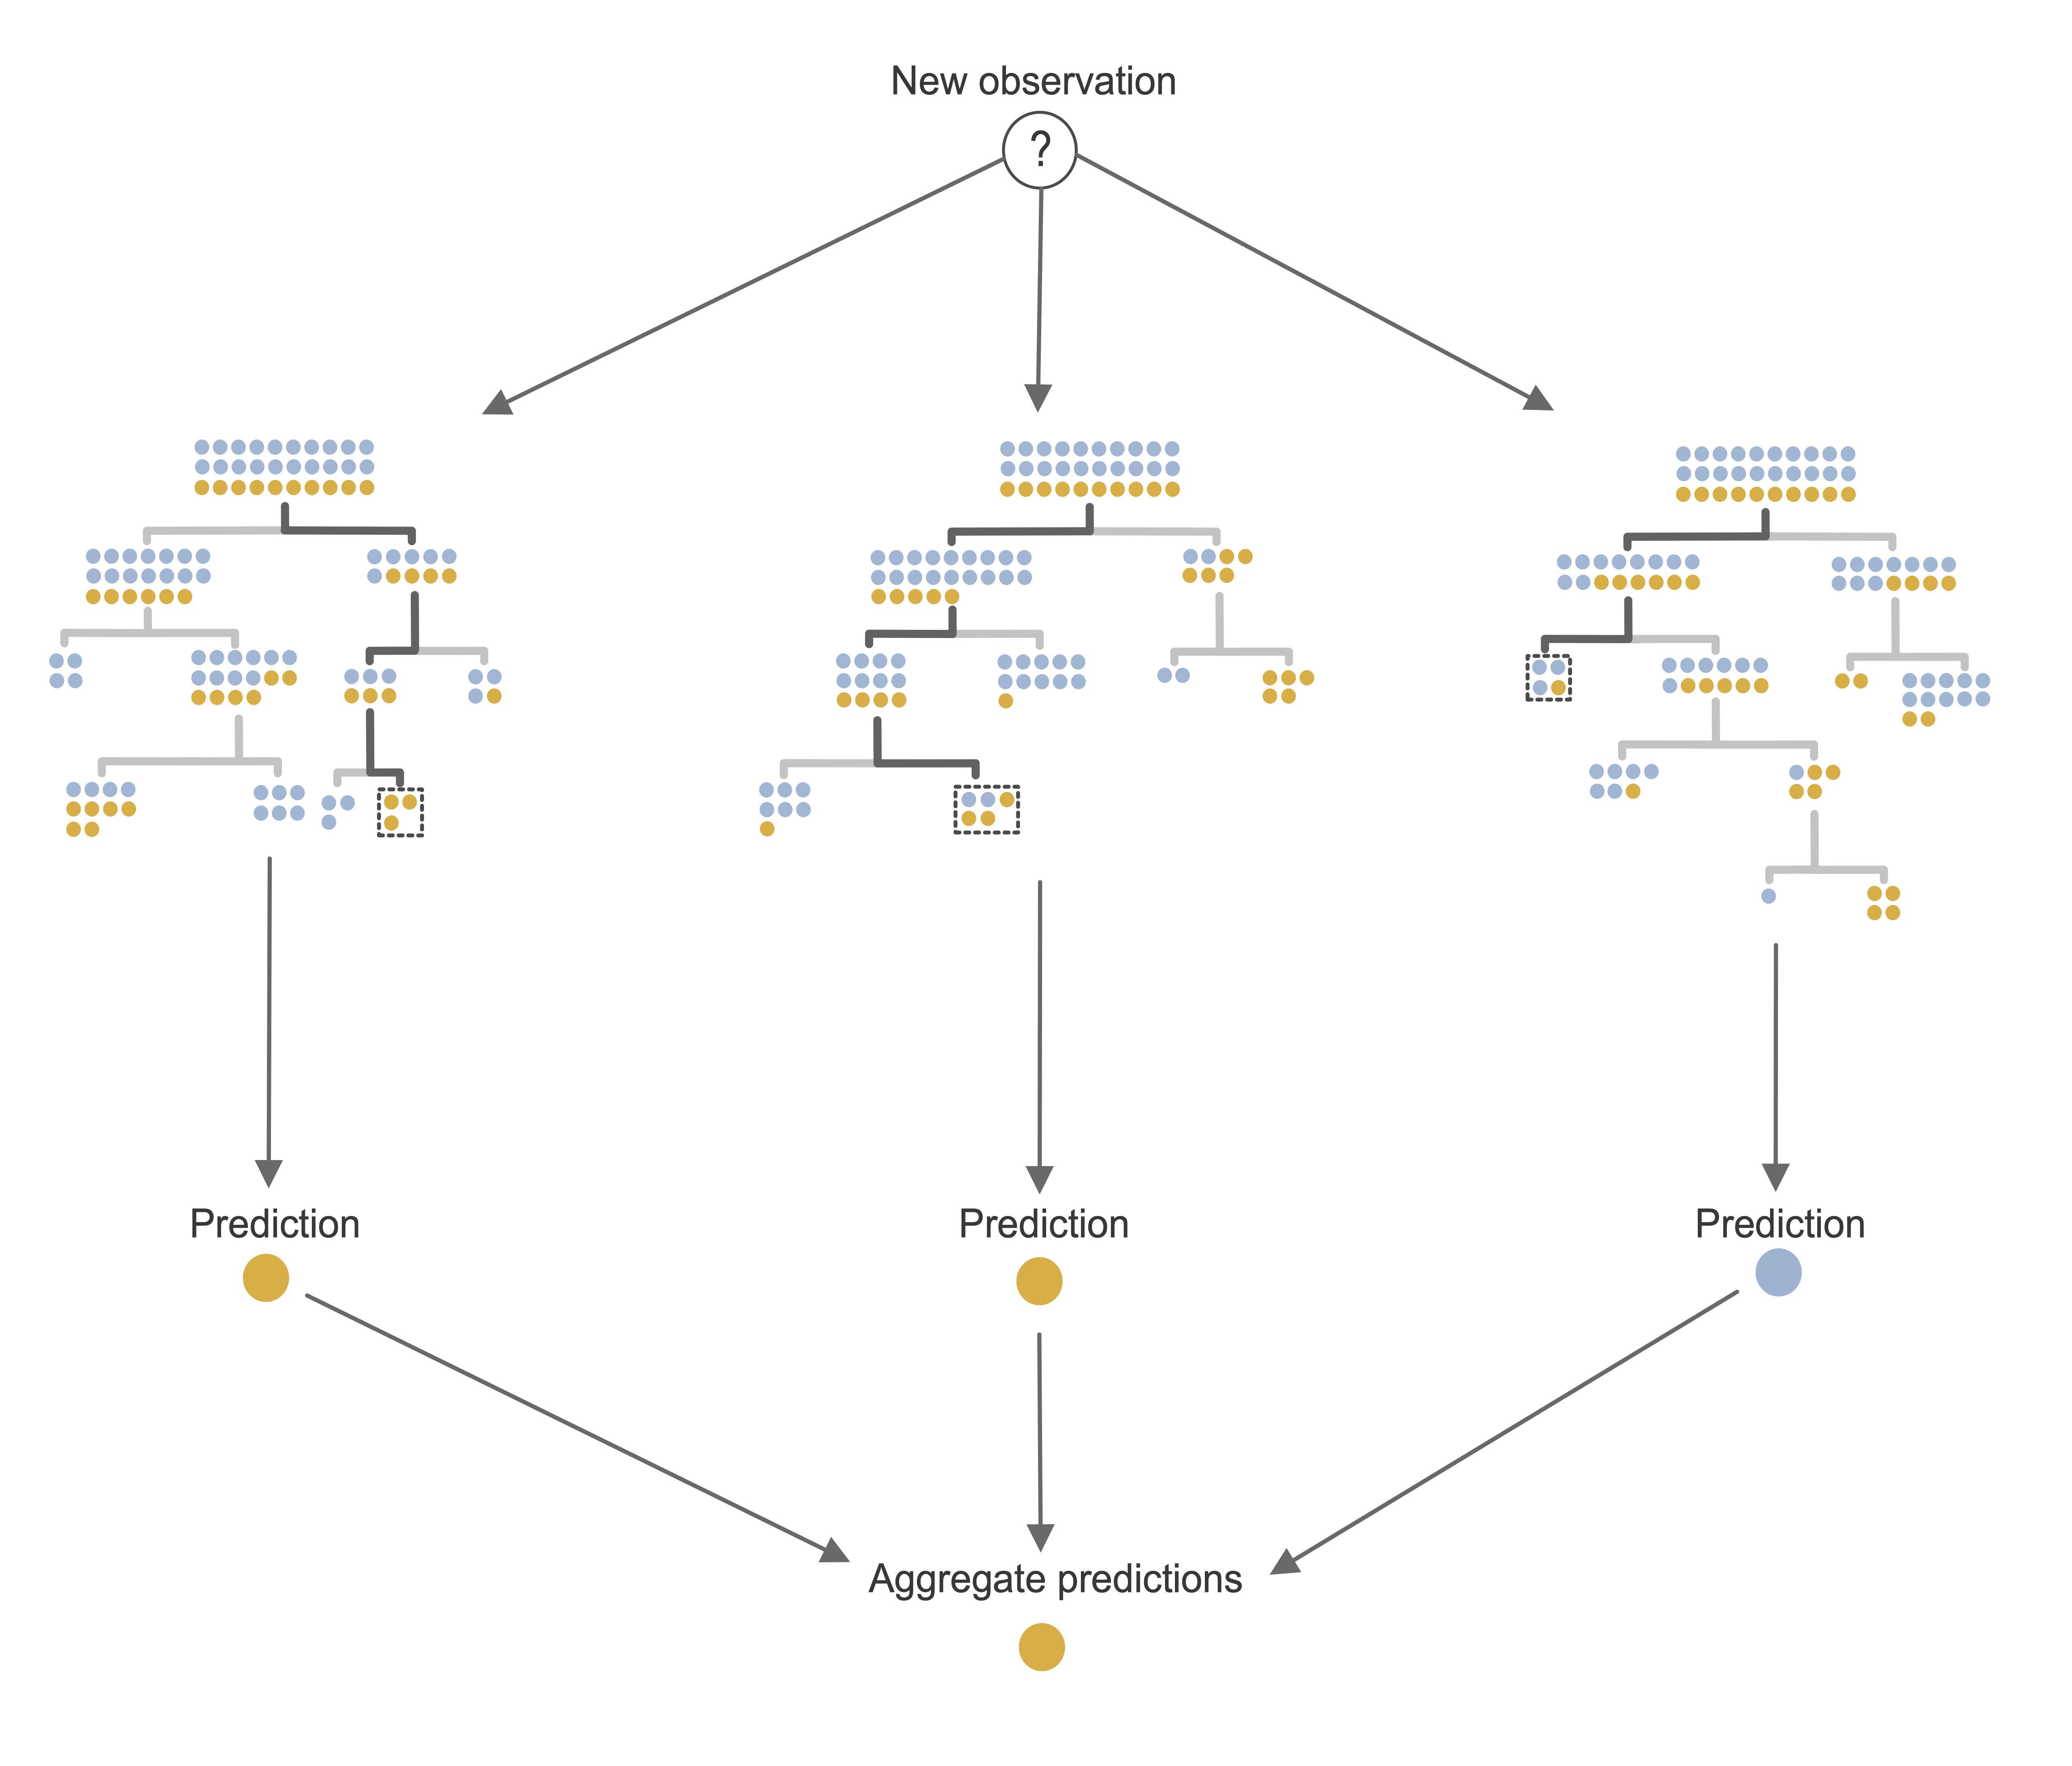
\includegraphics[width=0.6\textwidth]{../figures/random_forest_illustrated.png}
		\caption{An RF fit based on an ensemble of just three trees is depicted. Source: \url{https://vdsbook.com/12-rf}}
	\end{figure}
\end{frame}


\begin{frame}{Bagging vs. Random Forests}
	\textbf{Bagging}: Bootstrapping for creating various subsets of the training data and averaging predictions from trees built on these subsets. Each tree is built using all features at each split.
	\medskip

	\textbf{Random Forests} = Bagging + Random Feature Selection at Splits
	\vspace{0.2cm}

	\begin{figure}
		\centering
		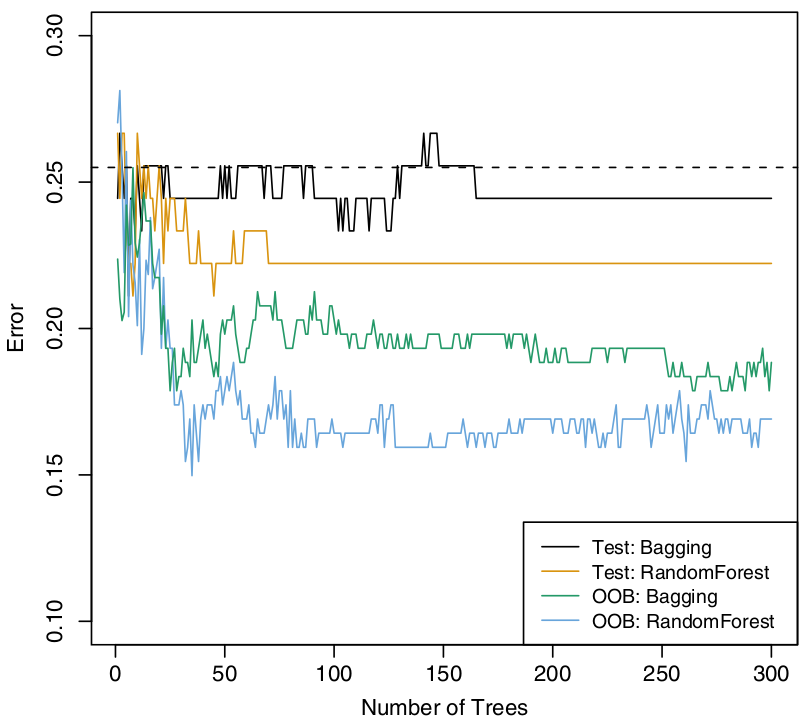
\includegraphics[width=.5\textwidth]{../figures/bagging_error_rate_decision_tree.png}
		\caption{\footnotesize The test error is a function of the number of bootstrap replications and thus trees, $B$. The black dashed line shows the test error of a single classification tree. Source: \citet[p. 318]{james2023IntroductionStatisticalLearning}.}
		\label{fig:bagging_error}
	\end{figure}
\end{frame}



\begin{frame}{Random Forests: Key Hyperparameters}
	\textbf{Main tuning parameters:}

	\begin{table}
		\tiny
		\begin{tabular}{|p{2.7cm}|p{3.2cm}|p{2.1cm}|p{2.3cm}|}
			\hline
			\textbf{Hyperparameter} & \textbf{Role} & \textbf{R (\texttt{ranger})} & \textbf{Python (\texttt{sklearn})} \\
			\hline
			Number of variables tried at each split &
			Controls randomness and tree diversity &
			\texttt{mtry} \newline default: $\lfloor \sqrt{p} \rfloor$ &
			\texttt{max\_features} \newline default: $\sqrt{p}$ \\
			\hline
			Maximum depth &
			Limits number of sequential splits; smaller depth regularizes &
			\texttt{max.depth} \newline default: unlimited &
			\texttt{max\_depth} \newline default: unlimited \\
			\hline
			Minimum node size /
			minimum samples to split &
			Stops further splitting in small nodes; larger values regularize &
			\texttt{min.node.size} \newline defaults depend on task &
			\texttt{min\_samples\_split} \newline default: 2 \\
			\hline
			Number of trees &
			More trees reduce variance but increase computation time &
			\texttt{num.trees} \newline default: 500 &
			\texttt{n\_estimators} \newline default: 100 \\
			\hline
		\end{tabular}
	\end{table}

	\vspace{0.2cm}

	\textbf{Practical takeaway:}
	\begin{itemize}
		\small
		\setlength{\itemsep}{0.1cm}
		\item Tune these hyperparameters using cross-validation
		\item In practice, default values often work reasonably well
		\item Start with defaults, then tune only if predictive performance needs improvement
	\end{itemize}
\end{frame}


\begin{frame}{Code Example 4: Random Forests in Gretl}

	See code examples:
	\vspace{0.25cm}

	\begin{itemize}
		\setlength{\itemsep}{0.15cm}
		\item \texttt{random\_forest\_regression.inp}: Random Forest regression example using the \texttt{random\_forest} gretl package
	\end{itemize}

\end{frame}


\begin{frame}{Feature Importance}
	\begin{itemize}
		\item Individual trees are easy to interpret.
		\item But how do we evaluate the relevance of high-dimensional (multiple features) ensembles (multiple models)?
		\item The importance of a variable is measured by the average reduction in error achieved by using this variable for splits in the trees.
		\item Various importance measures exist, e.g.
		\begin{enumerate}
			\item permutation importance score
			\item Gini importance score
			\item Impurity-based feature importance (\href{https://scikit-learn.org/stable/auto_examples/inspection/plot_permutation_importance.html}{tends to overestimate the importance})
		\end{enumerate}
		\item Other measures include SHAP values, LIME, and partial dependence plots.
		\item Relevant topic, generally known under the term \emph{Explainable AI}.
	\end{itemize}
\end{frame}


\begin{frame}{Permutation Feature Importance Algorithm}
	\begin{enumerate}
		\item \textbf{Inputs:} Fitted predictive model, tabular dataset
		\item \textbf{Compute baseline performance:} Calculate reference score $S$ on unmodified data (e.g., accuracy, MSE etc.)
		\item \textbf{For each feature $X_j$:}
			  \begin{enumerate}
				  \item For $r = 1$ to $R$ repetitions:
						\begin{enumerate}
							\item Create corrupted dataset by randomly shuffling rows of only feature $X_j$
							\item Compute performance score $S_r^j$ on this corrupted data
						\end{enumerate}
				  \item Calculate importance $I_j$ for feature $X_j$ as the decrease in performance:
						\begin{equation}
							I_j = S - \underbrace{\frac{1}{R}\sum_{r=1}^{R}S_r^j}_{\text{avg. score of permuted data}}
						\end{equation}
			  \end{enumerate}
		\item \textbf{Result:} Higher importance value indicates more influential features
	\end{enumerate}
\end{frame}


\begin{frame}{Permutation Feature Importance Visualization}
	\begin{figure}
		\centering
		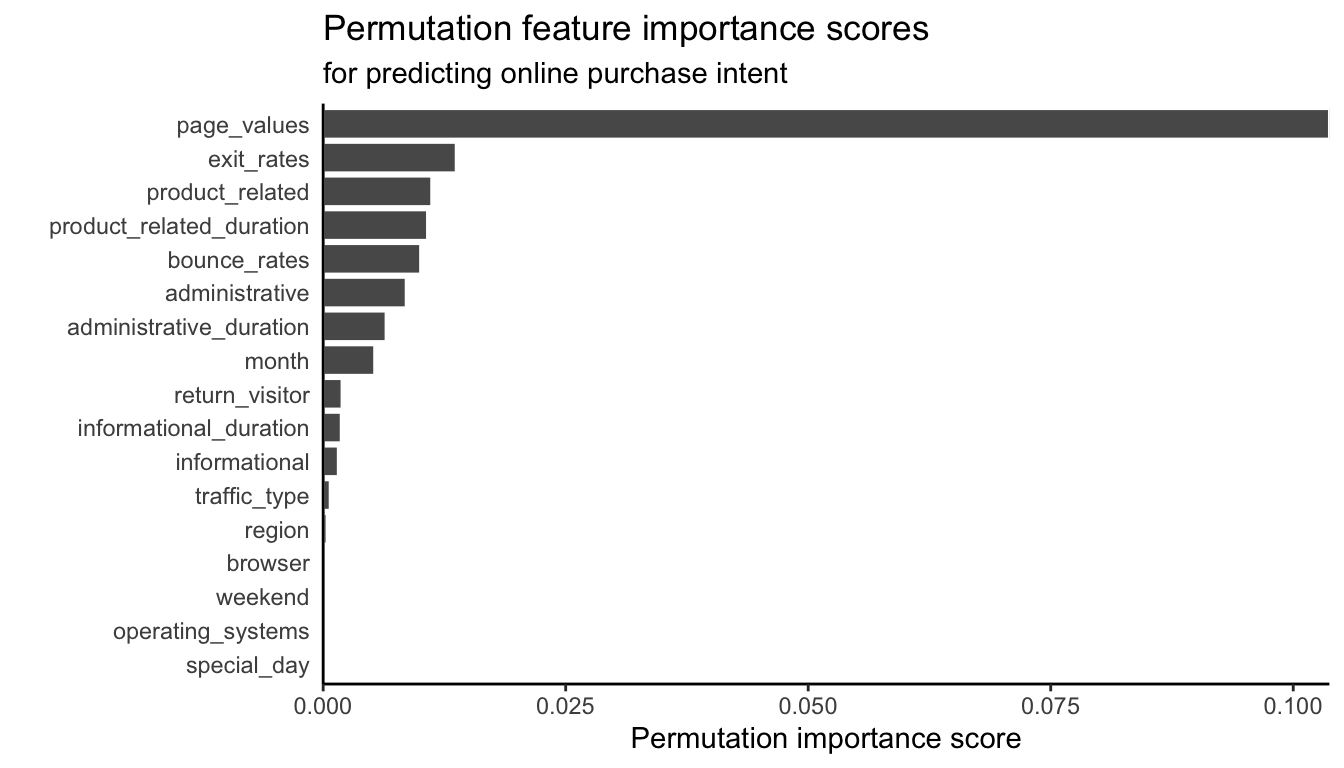
\includegraphics[width=.85\textwidth]{../figures/yu_barter_shopping-variable-importance-permutation.png}
		\caption{A bar chart showing the permutation feature importance of each variable in the RF fit for predicting online purchase intent. \footnotesize{Source: \url{https://vdsbook.com/12-rf\#fig-shopping-variable-importance-permutation}}}
	\end{figure}
\end{frame}


\begin{frame}{Gretl Package for Random Forests}
  \textbf{Package:} random\_forest.gfn \\
  \textbf{Author:} Allin Cottrell \\
  \textbf{Version:} 0.3 (December 2023) \\
  \textbf{Installation:} \texttt{pkg install random\_forest}

  \vspace{0.1cm}

  \textbf{Main Features:}
  \begin{itemize}
    \item Wraps R's \texttt{randomForest} package (requires R $\geq$ 4.1.0)
    \item Supports both regression and classification tasks
    \item Main function: \texttt{random\_forest(y, X, opts)}
    \item Feature importance scoring and visualization
    \item Flexible train/test split via \textit{n\_train} or dummy series
    \item Automatic hyperparameter tuning (mtry) via \texttt{tuneRF}
    \item GUI interface available%: Model $\to$ Robust Estimation $\to$ Random Forest
  \end{itemize}

  \vspace{0.1cm}

  \textbf{Key Functions:}
  \begin{itemize}
    \item \texttt{random\_forest()}: Train and predict with random forests
    \item \texttt{rf\_print()}: Display model results and feature importance
    \item \texttt{rf\_plot()}: Visualize feature importance (horizontal bar chart)
  \end{itemize}
\end{frame}


\begin{frame}{Boosting}
	\textbf{Question:} Can one combine multiple \textit{weak learners} in such a way that the ensemble becomes a \textit{strong learner}?\footnote{A weak learner is a simple model (in terms of complexity measured by the number of features, the degree of non-linearity or number of nodes in case of a tree) whose accuracy is just a little bit better than random guess.}
	\vfill

	\begin{itemize}
		\item Recall, bagging involves training each tree on a bootstrap data set, independent of the other trees.
		\item With boosting, each model is grown sequentially \textbf{using information from previously trained models}.
		\item Boosting combines multiple weak learners to produce a form of committee whose performance can be significantly better than that of any of the base classifiers $\Rightarrow$ Bias reduction
		\item Adaptive boosting (AdaBoost) is a strategy developed by \citet{Freund.Schapire1996} for classification.
		\item \citet{Friedman2001} introduced gradient-based boosting.
	\end{itemize}
\end{frame}


\section{Support Vector Machines}

\begin{frame}
	\begin{center}
		\Large
		Support Vector Machines (SVM)
	\end{center}
\end{frame}


\begin{frame}{Gretl Built-in SVM Functionality}
	\small
    \textbf{Author:} Allin Cottrell \\
  \textbf{Library:} libsvm (integrated plugin, no external installation needed)
  \textbf{Doc}: \url{https://sourceforge.net/projects/gretl/files/manual/gretl-svm.pdf}
  \vspace{0.1cm}

  \textbf{Main Features:}
  \begin{itemize}
    \item Built-in function: \texttt{svm(list L, bundle params)}
    \item Supports both regression and classification
    %\item Automatic type detection: binary/coded dependent variable $\to$ classification, else regression
    %\item Default kernel: RBF (Radial Basis Function); also supports linear, polynomial, sigmoid
    %\item Automatic feature scaling to $[-1,1]$ range (customizable)
    \item Flexible train/test split via \textit{n\_train} parameter
    \item Comprehensive cross-validation for hyperparameter tuning (grid/line search)
    %\item Probability estimation for predictions (regression error distribution, classification probabilities)
    \item MPI support for large-scale parallel cross-validation
  \end{itemize}

  \vspace{0.1cm}

  \textbf{Key SVM Types \& Kernels:}
  \begin{itemize}
    \item Classification: C-SVC (cost-based) or \textit{$\nu$}-SVC (fraction of support vectors)
    \item Regression: \textit{$\epsilon$}-SVR (margin-based) or \textit{$\nu$}-SVR (support vector fraction)
    \item Kernels: linear, polynomial (with degree parameter), RBF, sigmoid
  \end{itemize}
\end{frame}


\begin{frame}[fragile]{Tree-Based vs. Kernel Methods: Comparison}
	\begin{table}
		\scriptsize
		\centering
		\setlength{\tabcolsep}{4pt}
		\renewcommand{\arraystretch}{1.15}
		\begin{tabular}{|p{0.22\textwidth}|p{0.34\textwidth}|p{0.34\textwidth}|}
			\hline
			\textbf{Aspect} & \textbf{Trees / Random Forests} & \textbf{Kernel Methods (SVM, KNN)} \\
			\hline
			Interpretability & High & Low \\
			\hline
			Feature importance & Built-in (Gini, permutation) & Difficult to extract \\
			\hline
			Computational cost & Moderate & High (especially SVM) \\
			\hline
			Nonlinearity & Automatic (recursive splits) & Via kernel choice \\
			\hline
			Scaling features & Not necessary & Essential \\
			%\hline
			%High dimensions & Possible & Better (with RBF kernel) \\
			\hline
			Interaction effects & Captures naturally & Needs manual specification \\
			\hline
		\end{tabular}
	\end{table}

	\vspace{0.2cm}

	\textbf{Rule of thumb:}
	\begin{itemize}
		\small
		\setlength{\itemsep}{0.1cm}
		\item \textbf{Trees/RF}: Start here for interpretability, feature importance
		\item \textbf{SVM/KNN}: Try when trees underperform or the number of features is low
	\end{itemize}
\end{frame}


% \begin{frame}{Comparison of Machine Learning Methods}
% 	\begin{table}[ht]
% 		\centering
% 		\scriptsize
% 		\begin{tabular}{p{3.2cm}ccccc}
% 			\toprule
% 			\textbf{Characteristic}                            & \textbf{SVM}                        & \textbf{CART}                       & \textbf{GAM}                        & \textbf{KNN}                        & \textbf{Gradient Boost}             \\
% 			\midrule
% 			Natural handling of data of ``mixed'' type         & {\color{red}poor}                   & {\color{green}\checkmark\checkmark} & {\color{green}\checkmark\checkmark} & {\color{red}poor}                   & {\color{green}\checkmark\checkmark} \\
% 			\hline
% 			Handling of missing values                         & {\color{red}poor}                   & {\color{green}\checkmark\checkmark} & {\color{red}poor}                   & {\color{green}\checkmark\checkmark} & {\color{green}\checkmark\checkmark} \\
% 			\hline
% 			Robustness to outliers in input space              & {\color{red}poor}                   & {\color{green}\checkmark\checkmark} & \checkmark                          & {\color{green}\checkmark\checkmark} & {\color{green}\checkmark\checkmark} \\
% 			\hline
% 			Insensitive to monotone transformations of inputs  & {\color{red}poor}                   & {\color{green}\checkmark\checkmark} & {\color{green}\checkmark\checkmark} & {\color{red}poor}                   & {\color{green}\checkmark\checkmark} \\
% 			\hline
% 			Computational scalability (large $N$)              & {\color{red}poor}                   & {\color{green}\checkmark\checkmark} & {\color{green}\checkmark\checkmark} & {\color{red}poor}                   & {\color{green}\checkmark\checkmark} \\
% 			\hline
% 			Ability to deal with irrelevant inputs             & {\color{red}poor}                   & {\color{green}\checkmark\checkmark} & \checkmark                          & {\color{red}poor}                   & {\color{green}\checkmark\checkmark} \\
% 			\hline
% 			Ability to extract linear combinations of features & {\color{green}\checkmark\checkmark} & {\color{red}poor}                   & {\color{red}poor}                   & \checkmark                          & \checkmark                          \\
% 			\hline
% 			Interpretability                                   & {\color{red}poor}                   & \checkmark                          & {\color{green}\checkmark\checkmark} & {\color{red}poor}                   & {\color{green}\checkmark\checkmark} \\
% 			\hline
% 			Predictive power                                   & {\color{green}\checkmark\checkmark} & {\color{red}poor}                   & {\color{red}poor}                   & {\color{green}\checkmark\checkmark} & {\color{green}\checkmark\checkmark} \\
% 			\bottomrule
% 		\end{tabular}
% 		\caption{\footnotesize Comparison of characteristics across different machine learning methods.}
% 	\end{table}
% \end{frame}

% ==================== SECTION 4: CROSS-VALIDATION & EVALUATION ====================

\section{Cross-Validation and Model Evaluation}

\begin{frame}
	\begin{center}
		\Large
		Cross-Validation and Model Evaluation\\
		\vspace{0.5cm}
		\normalsize
		Robust Performance Assessment
	\end{center}
\end{frame}

\begin{frame}{Training and Test Errors}
    We distinguish between:
    \begin{enumerate}
        \item \textbf{Training error}: Average error between realization and prediction on the training data (\textit{In-Sample Error}).
        \item \textbf{Test (Generalization) error}: Average error when predicting unseen test data (also \textit{Out-of-Sample} prediction).
    \end{enumerate}
    \medskip

    \textbf{Goal}: The test error should be as small as possible.
    \medskip

    The training error can dramatically underestimate the test error.
    \medskip

    For model selection and evaluation, estimate the test error.
\end{frame}


\begin{frame}[fragile]{Why Cross-Validation?}
	\begin{itemize}
		\setlength{\itemsep}{0.3cm}
		\item \textbf{Single test set problem}: With one split, results are unstable (depends on lucky/unlucky split)
		\item \textbf{Data scarcity}: May not have enough data to dedicate large portion to testing
		\item \textbf{Better generalization estimate}: Average error across multiple folds more reliable
		\item \textbf{Hyperparameter tuning}: Need unbiased estimate of performance for parameter selection
		\item \textbf{Model agnostic}: Works for any model
	\end{itemize}

	\vspace{0.3cm}

	\textbf{Core principle:} Avoid using the same data for training and evaluation
\end{frame}


\begin{frame}{k-Fold Cross-Validation \textbf{I}}
    \small
    \begin{columns}
        \begin{column}{0.55\textwidth}
            \begin{itemize}
                \item Split the available data into $k$ groups.
                \item $k-1$ of the groups are used to train a model.
                \item Evaluate the model on the remaining validation group using a <METRIC>.
                \item Repeat the steps for all $k$ (typically 5 or 10) possible choices.
                \item The calculated evaluation metrics are averaged to estimate the error rate.
                \item LOOCV is a special case of k-fold CV, where $k=n$.
        \end{itemize}
        \end{column}
        \begin{column}{0.45\textwidth}  %%<--- here
            % \begin{figure}
            % 	\centering
            % 	\subfigure{
            % 		\includegraphics[width=1.0\textwidth]{../figures/kfold_approach_k=4.png}}
            % 	\caption{\footnotesize{Illustration of k-fold CV for $k=4$. Data used for training is in white. The held-out set is indicated by the red block.}}
            % \end{figure}

            \begin{figure}
                \centering
                \subfigure{
                    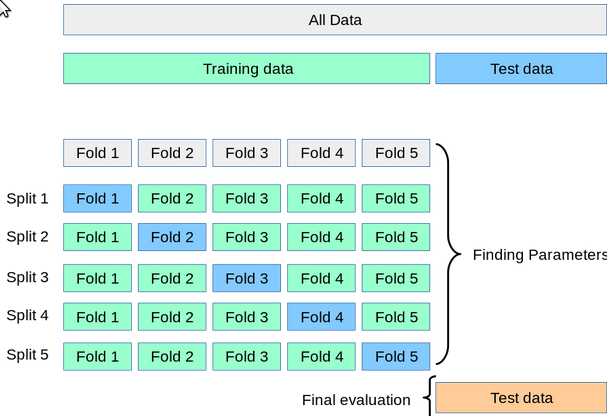
\includegraphics[width=1.0\textwidth]{../figures/kfold_approach_k=5_scikitlearn.png}}
                \caption{\footnotesize{Illustration of k-fold CV for $k=5$. The training data is shown in green. The held-out set is indicated by the blue block.}}
            \end{figure}
        \end{column}
    \end{columns}
\end{frame}


\begin{frame}{Comparison of LOOCV and k-Fold CV}
    \begin{figure}
        \centering
        \subfigure{
            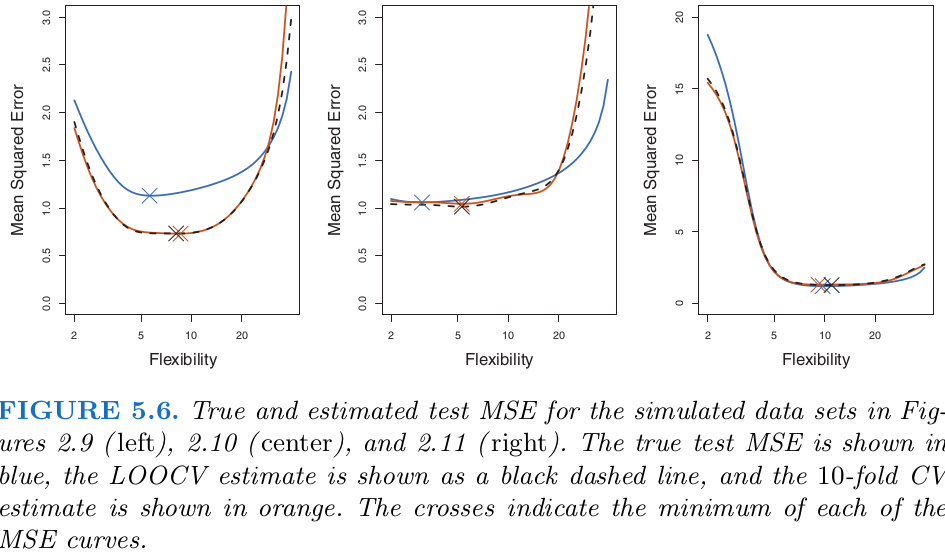
\includegraphics[width=0.8\textwidth]{../figures/kfold_loocv_comparison_James_etal_2017.png}}
        \caption{\footnotesize Similar test error rates achieved by LOOCV and $k$-fold CV. Even though the test error may be underestimated, the correct hyperparameter value that minimizes the MSE can be well estimated by CV. Source: \citet[p. 208]{james2023IntroductionStatisticalLearning}.}
    \end{figure}
\end{frame}



\subsection{CV for Classification Problems}


\begin{frame}{Classification Problems}
    \begin{itemize}
        \item CV is also useful for classification problems.
        \item The previously described CV techniques are analogous to what was described before.
        \item However, the loss function needs to change.
        \item For classification, we could calculate the classification error as follows:
        \begin{equation}
            e_i = \mathbf{1}(y_i \neq \hat y_i)
        \end{equation}
        which is known as "zero-one loss."
        \item The LOOCV test error rate then becomes:
        \begin{equation}
            CV_n = \frac{1}{n} \sum_{i=1}^n \mathbf{1}(y_i \neq \hat y_i)
        \end{equation}
    \end{itemize}
\end{frame}


\begin{frame}{Cross-Validation}
    \begin{figure}
        \centering
		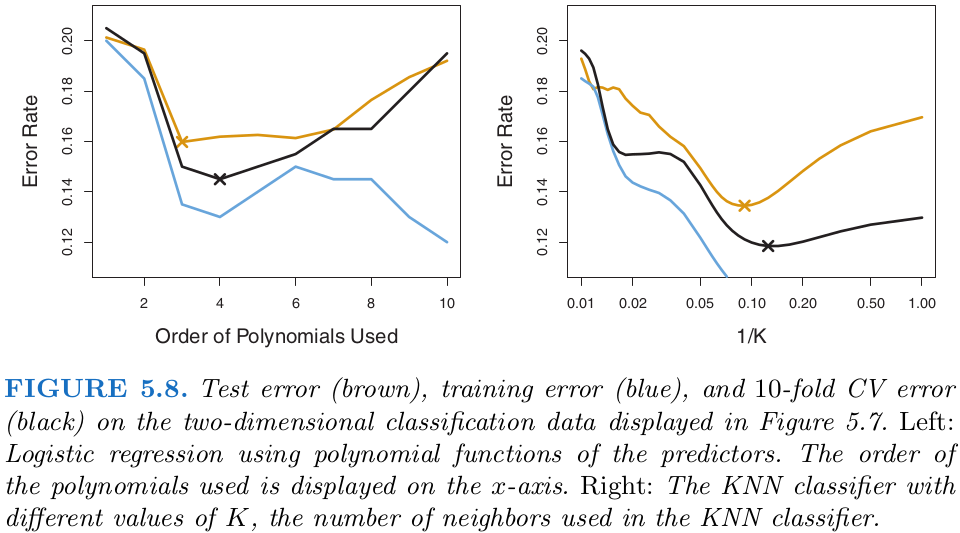
\includegraphics[width=0.9\textwidth]{../figures/kfold_classification_James_etal_2017.png}
        %\caption{\footnotesize Similar test error rates achieved by LOOCV and $k$-fold CV. Even though the test error may be underestimated, the correct hyperparameter value that minimizes the MSE can be well estimated by CV. Source: \citet[p. 186]{James.etal2017}.}
    \end{figure}
    Source: \citet[p. 211]{james2023IntroductionStatisticalLearning}
\end{frame}


\begin{frame}{Imbalanced Class Distribution}
    \begin{itemize}
        \item Some classification problems may have a large imbalance in the distribution of target classes.
        \item For example, there could be many times more negative than positive samples.
        \item In such cases, stratified sampling is used to ensure that the relative class frequencies are approximately preserved in each train and validation fold.
    \end{itemize}
	\vspace{0.3cm}

    $\Rightarrow$ Use stratified k-fold CV.
\end{frame}


\begin{frame}{Imbalanced Class Distribution}
    \begin{figure}
        \centering
		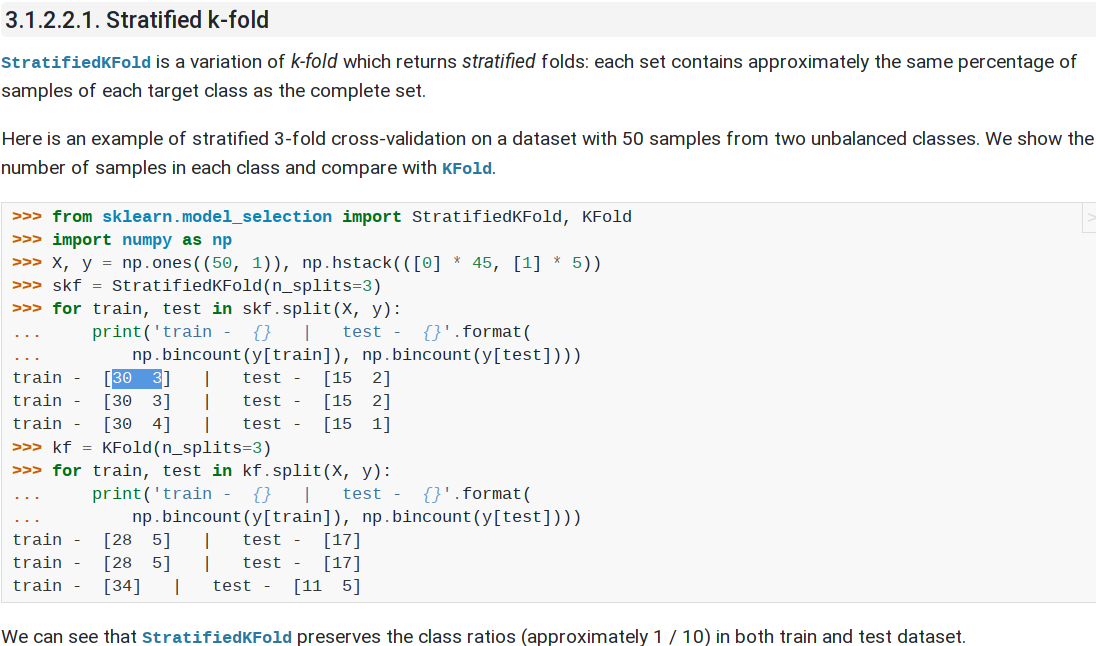
\includegraphics[width=0.85\textwidth]{../figures/kfold_stratified_scikitlearn.png}
    \end{figure}
    Source: \url{https://scikit-learn.org/stable/modules/cross_validation.html\#stratified-k-fold}
\end{frame}


\subsection{CV for Time-Series Problems}


\begin{frame}{Cross-Validation of Time Series Data (and Panel Data)}
    \small
    \begin{columns}
        \begin{column}{0.5\textwidth}
            \begin{itemize}
                \item Time series exhibit inherent serial correlation and are potentially non-stationary.
                \item Applying CV is not straightforward and is typically replaced by out-of-sample evaluation.
                \item The training set consists only of observations that occur before the period to be forecasted.
                \item Therefore, no future observations can be used when creating the forecast.
        \end{itemize}
        \end{column}
        \begin{column}{0.5\textwidth}  %%<--- here
            \begin{figure}
                \centering
				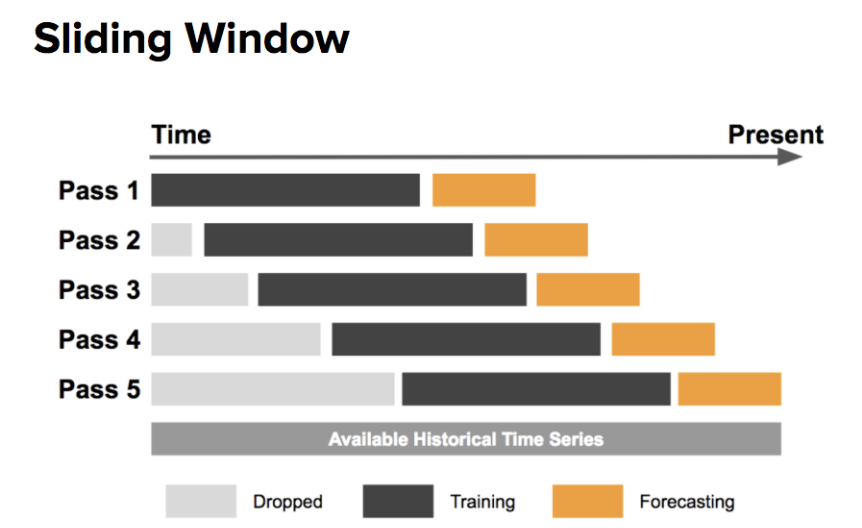
\includegraphics[width=1.0\textwidth]{../figures/uber_backtesting_sliding_window.png}
                \caption{\footnotesize{Cross-validation procedure with a 'rolling' window for training. The diagram shows a sequence of $h$-step ahead forecasts can be created.}}
            \end{figure}
        \end{column}
    \end{columns}
\end{frame}


\begin{frame}{CvDataSplitter Package for Cross-Validation Splits}
	\small
		\textbf{Author:} Artur Tarassow \\
	\textbf{Package:} \texttt{CvDataSplitter.gfn} (Version 0.3, 2021-06-21)
	\textbf{Doc}: \url{https://gretl.sourceforge.net/current_fnfiles/CvDataSplitter.gfn}
	\vspace{0.1cm}

	\textbf{Main Features:}
	\begin{itemize}
		\item Public function: \texttt{CvDataSplitter(\&b)} with bundle-based configuration
		\item Multiple CV strategies: \textit{kfold} (default), \textit{loo}, \textit{recwin}, and \textit{rolwin}
		\item Flexible input modes: pass predictors as a list or as a matrix (with index vector)
		\item User control via bundle options such as \textit{n\_folds} (for k-fold CV) and \textit{win\_size} (for time-window CV)
		\item Output prepared for modeling: train/test splits stored in arrays (e.g., \texttt{b.X\_train}, \texttt{b.X\_test})
	\end{itemize}
\end{frame}


\subsection{Evaluation Metrics for Regression}

\begin{frame}{Forecast Errors for Regression}
    \begin{itemize}
        \item Forecast error as the difference between the observed value $y_i$ and the forecast $\hat y_i$:
        \begin{equation}
            e_i = y_i - \hat y_i
        \end{equation}
        \item Decomposition of the error into different components: Forecast Error $=$ $\text{Bias}^2$ + Variance + Noise
        \item Forecast error does not mean 'error' in the sense of 'wrong'.
        \item Forecast errors represent the non-predictable part of the observations -- conditional the model is correctly specified.
        \item Measurement of forecast performance by summarizing forecast errors in different ways.
    \end{itemize}
\end{frame}


\begin{frame}{Evaluation Metrics for Regression}
	An overview of some metrics for measuring prediction accuracy:
	\medskip

	\begin{table}
		\small
		\begin{tabular}{|l|l|l|}
			\hline
			\textbf{Metric} & \textbf{Formula}                                            & \textbf{Interpretation}                    \\
			\hline
			ME 			& $\frac{1}{n} \sum (y_i - \hat{y}_i)$                         & Average error (bias)                      \\
			\hline
			RMSE		   & $\sqrt{\frac{1}{n} \sum (y_i - \hat{y}_i)^2}$                & Standard deviation of errors               \\
			\hline
			MAE             & $\frac{1}{n} \sum |y_i - \hat{y}_i|$                        & Average absolute error                     \\
			\hline
			MAPE			& $\frac{100\%}{n} \sum \left| \frac{y_i - \hat{y}_i}{y_i} \right|$ & Average percentage error (scale-free) \\
			\hline
		\end{tabular}
	\end{table}
	\vspace{0.25cm}

	For discussions on the advantages and disadvantages of each metric, see \citet{hyndman2006AnotherLookMeasures,hyndman2014MeasuringForecastAccuracy}.
\end{frame}

\subsection{Evaluation Metrics for Classification}

\begin{frame}{Metrics for Classification Problems}
    \begin{itemize}
        \item There are many different metrics for evaluating classification performance.
        \item The choice depends, among other things, on whether it's a binary or multi-class classification problem.
        \item Libraries:
			\begin{itemize}
				\item Python: \texttt{sklearn.metrics} module
				\item Gretl: \texttt{FEP} package
			\end{itemize}
        \item Measures assume that the predictions are either:
        \begin{itemize}
            \item binary (0/1) or multi-class (e.g., 0, 1, 2, ...), or
            \item probabilities (e.g., $P(y=1|x)$).
        \end{itemize}
    \end{itemize}
\end{frame}


\begin{frame}{Binary Classification: Evaluation Metrics}
    \begin{center}
		\scriptsize
        \begin{tabular}{c|c|c|c}
            & \textbf{Predicted} & & \\
            \textbf{Observed} & 0 & 1 & \textbf{Total} \\
            \hline
            0 & TN & FP & $N^\ast$ \\
            \hline
            1 & FN & TP & $P^\ast$ \\
            \hline
            \textbf{Total} & $N^\ast$ & $P^\ast$ & $N + P$ \\
            \hline
        \end{tabular}
    \end{center}

    \vspace{0.2cm}
    \begin{table}
        \scriptsize
        \begin{tabular}{|l|l|}
            \hline
            \textbf{Metric}      & \textbf{Definition}                                                                                      \\
            \hline
            Accuracy             & $\frac{\text{TP} + \text{TN}}{\text{TP} + \text{TN} + \text{FP} + \text{FN}}$ = fraction correct         \\
            \hline
            Precision            & $\frac{\text{TP}}{\text{TP} + \text{FP}}$ = of predicted positives, how many correct?                    \\
            \hline
            Recall (Sensitivity) & $\frac{\text{TP}}{\text{TP} + \text{FN}}$ = of actual positives, how many detected?                      \\
            \hline
            Specificity          & $\frac{\text{TN}}{\text{TN} + \text{FP}}$ = of actual negatives, how many correctly rejected?            \\
            \hline
            F1-Score             & $2 \cdot \frac{\text{Precision} \times \text{Recall}}{\text{Precision} + \text{Recall}}$ = harmonic mean \\
            \hline
        \end{tabular}
    \end{table}

    \vspace{0.1cm}
    \textbf{Where:}
    \begin{itemize}
        \item TP = True Positives, TN = True Negatives
        \item FP = False Positives, FN = False Negatives
    \end{itemize}

    \vspace{0.1cm}
    \textbf{Trade-off:} Precision vs. Recall depends on context
    \begin{itemize}
        \small
        \item High recall: Medical diagnosis (minimize missed cases)
        \item High precision: Spam filtering (avoid false alarms)
    \end{itemize}
\end{frame}


\begin{frame}{From Binary to Multi-class and Multi-label Classification}
    \begin{itemize}
        \item Some metrics are primarily for binary classification tasks (e.g., F1-Score, ROC AUC).
        %\item By default, only the positive label is evaluated (usually label 1, can be configured using pos\_label).
        \item In multi-class or multi-label problems, the data is treated as a collection of binary problems.
        \item There are different methods to average binary metrics across multiple classes:
        \begin{itemize}
            \item \textbf{macro}: Calculates the average of binary metrics with equal weight for each class. Useful when rare classes are important.
            \item \textbf{weighted}: Accounts for class imbalance by weighting each class according to its frequency in the true data.
            \item \textbf{micro}: Gives each sample-class pair equal contribution to the overall metric. Sums the numerators and denominators of class metrics.
            \item \textbf{samples}: Only for multi-label problems. Calculates the metric over the true and predicted classes for each sample.
        \end{itemize}
		\item See \citet[pp. 197]{raschka2019PythonMachineLearning} and \url{https://scikit-learn.org/stable/modules/model_evaluation.html\#from-binary-to-multiclass-and-multilabel}
    \end{itemize}
\end{frame}


\section{Unsupervised Learning: Clustering}

\begin{frame}
	\begin{center}
		\Large
		Unsupervised Learning\\
		\vspace{0.5cm}
		\normalsize
		K-Means Clustering and Determining Optimal $k$
	\end{center}
\end{frame}

\begin{frame}[fragile]{K-Means Clustering: Algorithm}
	\textbf{Goal:} Partition $n$ observations into $k$ clusters based on similarity

	\vspace{0.2cm}

	\textbf{K-Means Algorithm:}
	\begin{enumerate}
		\setlength{\itemsep}{0.15cm}
		\item Randomly initialize $k$ cluster centroids $\boldsymbol{\mu}_1, \ldots, \boldsymbol{\mu}_k$
		\item Repeat until convergence:
		      \begin{itemize}
			      \small
			      \item \textbf{Assignment step}: Assign each observation to closest centroid
			            \[
				            C_k = \{ i : \|\mathbf{x}_i - \boldsymbol{\mu}_k\| \leq \|\mathbf{x}_i - \boldsymbol{\mu}_{k'}\| \text{ for all } k' \neq k \}
			            \]
			      \item \textbf{Update step}: Recompute centroids as mean of assigned points
			            \[
				            \boldsymbol{\mu}_k \leftarrow \frac{1}{|C_k|} \sum_{i \in C_k} \mathbf{x}_i
			            \]
		      \end{itemize}
		\item Converged when assignments no longer change
	\end{enumerate}

	\vspace{0.2cm}

	\textbf{Minimizes:} Within-cluster sum of squares (WCSS)
	\[
		W = \sum_{k=1}^K \sum_{i \in C_k} \|\mathbf{x}_i - \boldsymbol{\mu}_k\|^2
	\]
\end{frame}


\begin{frame}{Illustration of the iterations}
	\begin{figure}
		\centering
		\subfigure{
			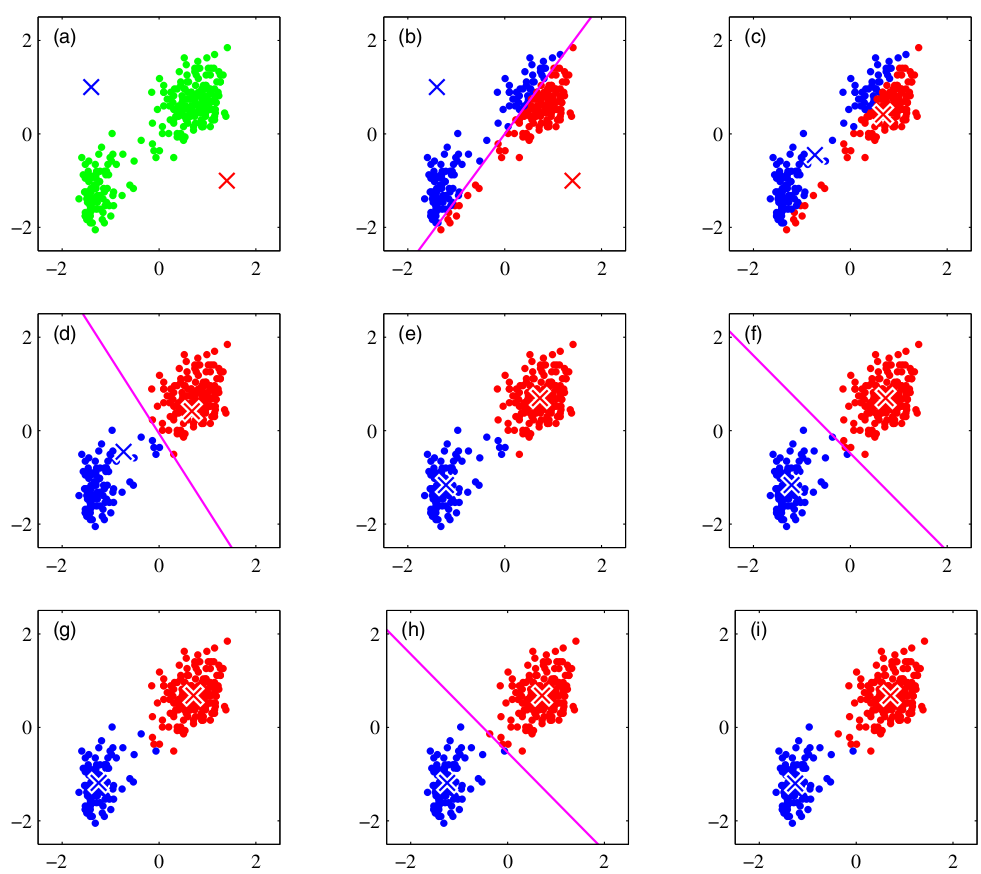
\includegraphics[width=.58\textwidth]{../figures/kmeans_iterations_from_bishop.png}}
		\caption{\footnotesize Illustration of the K-means algorithm for $K=2$ clusters. The centroids are shown as crosses. The algorithm quickly converges to a stable solution. Source: \citet{Bishop2016}.}
		\label{fig:kmeans_steps}
	\end{figure}
\end{frame}

\begin{frame}{K-Means: Common Distance Metrics}
	\begin{itemize}
		\setlength{\itemsep}{0.15cm}
		\item \textbf{Euclidean} (Default): $\|\mathbf{x}_i - \boldsymbol{\mu}_k\| = \sqrt{\sum_j (x_{ij} - \mu_{kj})^2}$ \newline
		  Use when: Features are continuous and on similar scales; assumes spherical clusters
		\item \textbf{Manhattan} (L1): $\sum_j |x_{ij} - \mu_{kj}|$ \newline
		  Use when: Less sensitive to outliers; works well with mixed feature types
		\item \textbf{Minkowski} (General): $\left(\sum_j |x_{ij} - \mu_{kj}|^p\right)^{1/p}$ \newline
		  Use when: $p=1$ is Manhattan, $p=2$ is Euclidean
		\item \textbf{Cosine}: $1 - \frac{\mathbf{x}_i \cdot \boldsymbol{\mu}_k}{\|\mathbf{x}_i\| \|\boldsymbol{\mu}_k\|}$ \newline
		  Use when: Text/document clustering; cares about direction, not magnitude
	\end{itemize}

	\vspace{0.2cm}

	\textbf{Important:} Always \textbf{standardize features} before clustering to avoid scale effects!
\end{frame}

\begin{frame}{K-Means: Initialization Problem}
	\textbf{Why Initialization Matters:}
	\begin{itemize}
		\setlength{\itemsep}{0.15cm}
		\item K-Means converges to \textbf{local optimum}, not global optimum
		\item Different random starting centroids $\Rightarrow$ different final solutions
		\item Quality of solution depends on initial placement
	\end{itemize}

	\vspace{0.3cm}

	\textbf{Solutions:}
	\begin{itemize}
		\setlength{\itemsep}{0.15cm}
		\item \textbf{Multi-run strategy}: Run k-means multiple times with different random seeds, keep best (smallest WCSS)
		\item \textbf{K-Means++}: Smarter initialization --- spread initial centroids far apart using probability-based selection
		\item \textbf{Domain knowledge}: Initialize centroids based on subject-matter expertise
	\end{itemize}
\end{frame}


\begin{frame}{How many clusters?}
	\begin{itemize}
		\item As clusters are \textbf{latent}.
		\item Widely used are \textit{ad hoc} heuristics such as the 'elbow method'.\footnote{For critique on the Elbow method, see e.g.\ \citet{schubert2023StopUsingElbow} and \citet[Ch. 12.4]{james2023IntroductionStatisticalLearning}.}
	\end{itemize}

	\begin{columns}[T,onlytextwidth]
		\begin{column}{0.42\textwidth}
			\textbf{Intuition:}
			\begin{itemize}
				\setlength{\itemsep}{0.15cm}
				\item WCSS always decreases as $k$ increases (more clusters fit data better)
				\item But improvement becomes marginal beyond optimal $k$
			\end{itemize}
		\end{column}
		\begin{column}{0.58\textwidth}
			\begin{figure}
				\centering
				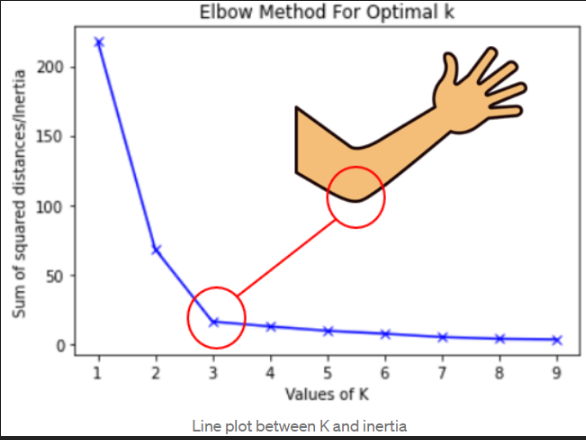
\includegraphics[width=0.7\textwidth]{../figures/kmeans_elbow_method.png}
				\caption{\footnotesize Elbow = point where marginal improvement drops off.}
				%\label{fig:kmeans_steps}
			\end{figure}
		\end{column}
	\end{columns}
\end{frame}


\begin{frame}[fragile]{Silhouette Plot: A Quantitative Approach}
	\textbf{Silhouette Coefficient:} Measures how similar an observation is to its own cluster vs. other clusters

	\vspace{0.1cm}

	For observation $i$:
	\begin{equation}
		s_i = \frac{b_i - a_i}{\max(a_i, b_i)}
	\end{equation}
	where:
	\begin{itemize}
		\small
		\setlength{\itemsep}{0.1cm}
		\item $a_i$ = average distance from $i$ to points in same cluster
		\item $b_i$ = average distance from $i$ to points in nearest other cluster
	\end{itemize}

	\vspace{0.cm}

	\textbf{Interpretation:}
	\begin{itemize}
		\setlength{\itemsep}{0.15cm}
		\item $s_i$ ranges from $-1$ to $+1$
		\item $s_i \approx +1$: Well-clustered (far from other clusters)
		\item $s_i \approx 0$: On boundary between clusters
		\item $s_i \approx -1$: Possibly misclassified
	\end{itemize}

	\vspace{0.2cm}

	\textbf{Use:} Silhouette plot shows $s_i$ for all observations; choose $k$ that maximizes average silhouette width.
\end{frame}


\begin{frame}{The 'kmeans' Gretl package}
	\textbf{Author}: Artur Tarassow\\
	\textbf{Installation:} \texttt{pkg install kmeans}
	\medskip

	\textbf{Main Features:}
	\begin{itemize}
		\item Implements the k-means clustering algorithm.
		\item Provides functions to perform k-means clustering on datasets, allowing users to specify the number of clusters and other parameters.
		\item The package includes functions
		\begin{itemize}
			\item for visualizing the clustering results,
			\item various distance metrics, and
			\item evaluating the quality of the clusters formed by means of Silhouette scores.
		\end{itemize}
		\item Documentation: \url{https://gretl.sourceforge.net/current_fnfiles/kmeans.gfn}
	\end{itemize}
\end{frame}


\begin{frame}{Questions?}
	\begin{center}
		\Large
		Thank you!
		\vspace{1cm}

		\normalsize
		Questions and Discussion
	\end{center}
\end{frame}

% ==================== APPENDIX: BIBLIOGRAPHY ====================

\begin{frame}[allowframebreaks]{Bibliography}
	\printbibliography
\end{frame}


% Appendix starts here
\appendix
% reset section numbering for appendix
\setcounter{section}{0}
% reset frame numbering for appendix
\setcounter{framenumber}{0}

\begin{frame}
	\begin{center}
		\Large
		Appendix
	\end{center}
\end{frame}

\begin{frame}{Loss Functions and Objective}
	\textbf{Different loss functions for different goals:}

	\vspace{0.2cm}

	\begin{table}
		\footnotesize
		\centering
		\setlength{\tabcolsep}{4pt}
		\renewcommand{\arraystretch}{1.15}
		\begin{tabular}{|p{0.22\textwidth}|p{0.36\textwidth}|p{0.34\textwidth}|}
			\hline
			\textbf{Method} & \textbf{Loss Function} & \textbf{Interpretation} \\
			\hline
			OLS & $\sum_{i=1}^n (y_i - \hat{y}_i)^2$ & Squared error \\
			\hline
			Robust Regression & $\sum_{i=1}^n |y_i - \hat{y}_i|$ & Absolute error (less sensitive to outliers) \\
			\hline
			Logistic Regression & $-\sum \left[y_i \log(\hat{p}_i) + (1-y_i)\log(1-\hat{p}_i)\right]$ & Cross-entropy (classification) \\
			\hline
			Hinge Loss (SVM) & $\sum \max(0,\, 1 - y_i \hat{f}(x_i))$ & Margin-based (robust) \\
			\hline
		\end{tabular}
	\end{table}
\end{frame}


\begin{frame}{ROC Curve for Binary Classification \textbf{I}}
    \begin{itemize}
        \item ROC stands for 'Receiver Operating Characteristics' and originates from communication theory.
        \item The ROC curve is a common graphical representation to display the two types of errors for all possible thresholds $c$.
        \item The overall performance of a classifier is given by the area under the curve (AUC).
        \item The statistics can be applied independently of the classifier used.
        \item The AUC is 0.5 for a classifier that performs no better than random chance.
    \end{itemize}
\end{frame}


\begin{frame}{ROC Curve for Binary Classification \textbf{II}}
    \begin{figure}
        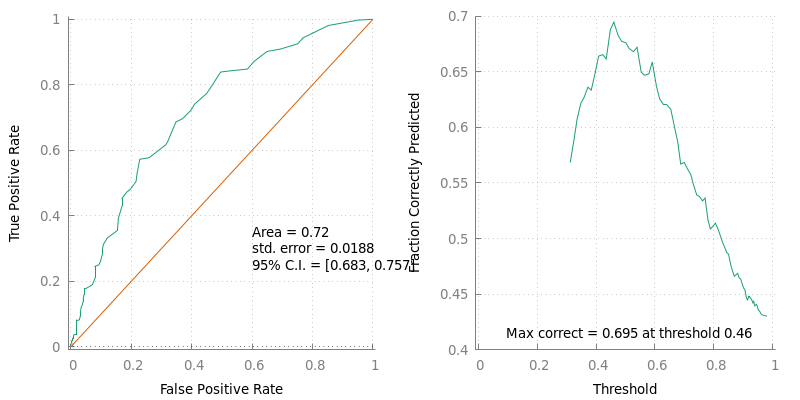
\includegraphics[scale=0.35]{../figures/mroz_logit_roc.png}
        \caption{\scriptsize A ROC curve for a Logit model with the \texttt{mroz87} data. \textbf{Left}: The curve traces two types of errors as the threshold $c$ varies. Each combination shows the true positive rate and false positive rate as a function of $c$. The ideal ROC curve hugs the upper left corner, showing a high true positive rate and a low false positive rate. The 45-degree line represents the 'no information' classifier (pure guessing). \textbf{Right}: This graph shows the proportion of correctly predicted classes as a function of the threshold parameter $c$. The maximum is reached at $c = 0.46$, which is only slightly different from the standard threshold of 0.5.}
    \end{figure}
\end{frame}


\begin{frame}{Brier Score Loss for Probabilistic Classification}
    \small
    \begin{itemize}
        \item The Brier Score (BS) loss function is applicable for binary classes.
        \item The BS is a "proper score function" that measures the accuracy of probabilistic predictions.
        \item The function calculates the mean squared error between the actual outcome and the predicted probability estimate.
        \item The value is between 0 and 1, with a lower value (smaller mean squared difference) indicating a more accurate prediction.
    \end{itemize}
    \begin{equation}
        \text{Brier Score} = \frac{1}{n} \sum_{i=1}^{n} (y_i - p_i)^2
    \end{equation}
    where $p=\Pr(y=1)$ and $y \in \{0,1\}$.
    \medskip

    \small{sklearn method: \url{https://scikit-learn.org/stable/modules/model_evaluation.html\#brier-score-loss}}
\end{frame}


\begin{frame}{SVM}
	\begin{center}
		\LARGE
		Support Vector Machines (SVM)
	\end{center}
\end{frame}

\begin{frame}[fragile]{Support Vector Machines (SVM): Core Idea}
	\textbf{Goal:} Find a separating hyperplane that maximizes the margin between classes.

	\vspace{0.1cm}

	\textbf{Linear SVM (for separable data):}
	\begin{equation}
		\min_{\boldsymbol{\beta}, b} \frac{1}{2} \|\boldsymbol{\beta}\|^2 \quad \text{subject to} \quad y_i(\mathbf{x}_i^\top \boldsymbol{\beta} + b) \geq 1 \text{ for all } i
	\end{equation}

	\begin{itemize}
		%\setlength{\itemsep}{0.15cm}
		\item \textbf{Margin}: Distance from hyperplane to nearest points (support vectors)
		\item Maximize margin $\Leftrightarrow$ minimize $\|\boldsymbol{\beta}\|^2$
		\item Support vectors are critical observations; ignore far points
	\end{itemize}

	\vspace{0.2cm}

	\textbf{Non-separable case (soft margin):}
	\begin{equation}
		\min_{\boldsymbol{\beta}, b, \boldsymbol{\xi}} \frac{1}{2} \|\boldsymbol{\beta}\|^2 + C \sum_{i=1}^n \xi_i
	\end{equation}

	\begin{itemize}
		%\setlength{\itemsep}{0.15cm}
		\item Allow misclassifications (slack variables $\xi_i$)
		\item Cost parameter $C$ trades off margin width vs. misclassification tolerance
	\end{itemize}
\end{frame}

% New slide depicting the maximum margin hyperplane and support vectors for classification
\begin{frame}
	\begin{figure}
		\centering
		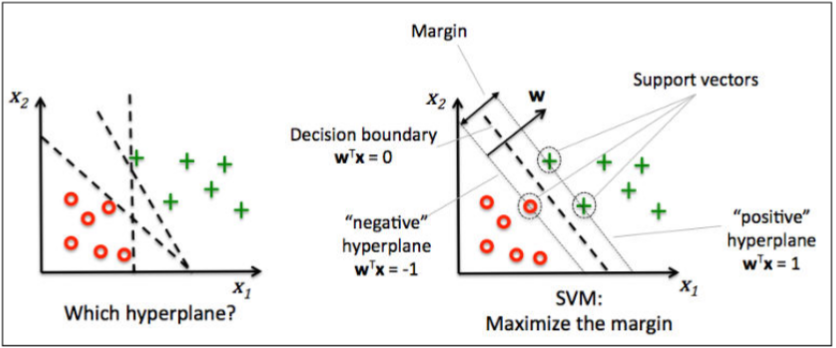
\includegraphics[width=0.7\textwidth]{../figures/raschka2019_classification_svm_maximum_margin.png}
		\caption{SVM margin and support vectors. Source: \citep[p. 69]{raschka2019PythonMachineLearning}.}
	\end{figure}
	\vspace{0.5cm}

	An open question in the field: Multiclass SVMs --- how to extend binary SVM to multi-class problems? Common approaches include one-vs-rest and one-vs-one strategies. For details, see \citet[p. 338]{Bishop2016}.
\end{frame}


\begin{frame}[fragile]{Support Vector Machines: Nonlinear Kernels}
	\textbf{Linear kernels work only for linearly separable data}

	\vspace{0.2cm}

	\textbf{Kernel Trick:} Transform data to high-dimensional space implicitly \citep[pp. 75]{raschka2019PythonMachineLearning}

	\vspace{0.2cm}

	\textbf{Common kernels:}
	\begin{table}
		\small
		\begin{tabular}{|l|l|l|}
			\hline
			\textbf{Kernel} & \textbf{Formula}                                                                        & \textbf{Use Case}     \\
			\hline
			Linear          & $K(\mathbf{x}_i, \mathbf{x}_j) = \mathbf{x}_i^\top \mathbf{x}_j$                        & Linearly separable    \\
			\hline
			Polynomial      & $K(\mathbf{x}_i, \mathbf{x}_j) = (\mathbf{x}_i^\top \mathbf{x}_j + r)^d$                & Moderate nonlinearity \\
			\hline
			RBF (Gaussian)  & $K(\mathbf{x}_i, \mathbf{x}_j) = \exp(-\gamma \|\mathbf{x}_i - \mathbf{x}_j\|^2)$       & Highly nonlinear      \\
			\hline
			Sigmoid         & $K(\mathbf{x}_i, \mathbf{x}_j) = \tanh(\kappa \mathbf{x}_i^\top \mathbf{x}_j + \theta)$ & Neural-inspired       \\
			\hline
		\end{tabular}
	\end{table}

	\vspace{0.2cm}

	\textbf{Hyperparameter tuning:} Kernel choice and parameters (e.g., $\gamma$, $d$) crucial --- select via cross-validation
\end{frame}

\begin{frame}[fragile]{SVM for Regression}
	\textbf{Support Vector Regression (SVR):} Similar to classification but predicts continuous values

	\vspace{0.2cm}

	\[
		\min_{\boldsymbol{\beta}, b, \boldsymbol{\xi}} \frac{1}{2} \|\boldsymbol{\beta}\|^2 + C \sum_{i=1}^n (\xi_i + \xi_i^*)
	\]

	subject to: $|y_i - (\mathbf{x}_i^\top \boldsymbol{\beta} + b)| \leq \varepsilon + \xi_i$ and similar for $\xi_i^*$

	\vspace{0.2cm}

	\begin{itemize}
		\setlength{\itemsep}{0.15cm}
		\item \textbf{Epsilon ($\varepsilon$)}: Insensitive zone --- errors $< \varepsilon$ are ignored (Hinge loss)
		\item \textbf{Sparse predictions}: Only observations outside $\varepsilon$ band are support vectors
		\item Particularly useful for high-dimensional regression
	\end{itemize}
\end{frame}

\end{document}